\documentclass[11pt]{article}
\usepackage[T1]{fontenc}
\usepackage{lmodern}
\usepackage{microtype}
\usepackage{amsmath,amssymb}
\usepackage[margin=1in]{geometry}
\usepackage{graphicx}
\usepackage{booktabs}
\usepackage{tabularx}
\usepackage{xltabular}
\usepackage{enumitem}
\usepackage{xcolor}
\usepackage{textcomp}
\usepackage{listings}
\usepackage{caption}
\usepackage{float}
\usepackage[colorlinks=true,linkcolor=blue!50!black,citecolor=blue!50!black,urlcolor=blue!50!black]{hyperref}
\hypersetup{pdftitle={Building data for ARC},pdfauthor={Russell Kirk}}

\graphicspath{{../figures/}}

\lstdefinestyle{code}{
  basicstyle=\ttfamily\small,
  columns=fullflexible,
  keepspaces=true,
  frame=single,
  rulecolor=\color{black!30},
  backgroundcolor=\color{black!3},
  commentstyle=\color{black!55}\itshape,
  keywordstyle=\color{blue!55!black},
  stringstyle=\color{red!50!black},
  showstringspaces=false,
  upquote=true,
  breaklines=true,
  xleftmargin=0.5em,
  xrightmargin=0.5em,
}
\lstdefinelanguage{Racket}[]{Lisp}{
  morekeywords={define,lambda,let,let*,for/list,for*/list,in-range,in-list,filter,sort,length,range,cond,if,and,or,rule!},
}
\lstset{style=code}

\newcommand{\todo}[1]{\textcolor{red!70!black}{\textbf{TODO:} #1}}
\newcommand{\gen}[1]{\texttt{#1}}

\title{Building data for ARC}
\author{Russell Kirk \\ \href{mailto:definitely.not.russell.kirk@gmail.com}{\texttt{definitely.not.russell.kirk@gmail.com}}}
\date{November 2026}

\begin{document}
\maketitle

\begin{abstract}
A synthetic ARC task is useful only if its label is correct and its
demonstrations determine that label. Volume fixes neither. Correct labels come
cheaply from executable rules; most of the work is making better lessons, that
is, choosing which demonstrations a learner sees together. We describe
ARCpuzzles, a library of 4,061 procedural generators for ARC-style tasks, of
which 1,984 are approved for training. We release all of it rather than a
curated top subset, unfinished generators included, each with its label and
evidence, so that others can use it and see how much work remains; this paper
describes the approved generators, how to use them, and the ideas and pitfalls
we met in building them. Each generator pairs a Python input
sampler with a reference rule in a Racket DSL that computes every label, and
can declare what teaches its rule and what hides it. A generator can use the sample
number to choose what kind of input to draw next, so that successive draws rule
out named rival rules; 1,007 approved generators do. 1,352 approved generators
declare rivals, and at least 761
declare \emph{canonical shortcuts}, rival rules that reproduce every pair of the
original task, test included, but differ from the intended rule elsewhere; a gate added late in the
project verifies that declaration, and some approved generators fail it. 941 accepted parametric
families add 1,233 Racket rule variants, and each of their lessons must show
which variant produced it. Training takes only approved generators, whose approval is bound to the
reviewed source; a twelve-stage check battery, each stage added after a defect
found in review, runs alongside review, and approved generators are not
re-checked when a stage is added. We define four verification properties (consistent, grounded,
identifiable, reviewed) and show that agreement between label programs, the
check used by RE-ARC and NVARC, does not imply identifiability: a
commit--reveal blind solve finds an NVARC puzzle whose first four
demonstrations fit a second rule that is wrong on 17 of its 30 pairs, and an
identifiability screen asks for extra demonstrations on 2--4\% of RE-ARC,
ARC-GEN and NVARC episodes and flags 1.8\% of ARCpuzzles episodes, which, unlike the
external episodes, were not screened before training. Our ARC-AGI-2 submission, a Qwen3.8-27B trained for
273 GPU-hours on these data, is reported in the appendix, with per-generator
mastery measured on fresh draws by reading the model's probability of every
answer token (prefill scans).
\todo{release link and final score.}
\end{abstract}

\section{Introduction}
\label{sec:intro}

An ARC-AGI-2 puzzle is implicitly a function $f$ from grids to grids. A solver
sees a few input/output pairs, the demonstrations, and has to infer $f$ from
them to answer a test input, the query. We call the demonstrations together
with the query input a \emph{lesson}. ARCpuzzles works in the opposite
direction: it starts from $f$ and produces the pairs. For each puzzle it writes
$f$ explicitly as a small Racket program. It then asks a second question: which
input grids show the rule at work, and which hide it, for example an input on
which the rule changes nothing? Each generator answers that question in the
Python code that draws its inputs. Outputs are never written by hand; they are
computed by running $f$ on the generated input.

NVARC and the 2026 third-place ARC-AGI-2 solution train models on synthetic
puzzles at scale \cite{nvarc,darragh2026}. Their checks ask whether several
independently written programs agree on each output. Agreement is evidence that
an output follows the author's intended rule. It is not evidence that the
demonstrations shown to the learner determine that rule: if a simpler rival
rule also fits every demonstration but gives a different answer on the query,
the lesson is ambiguous however consistent its labels are.

No finite set of demonstrations determines a rule uniquely. For demonstrations
$D=\{(x_i,f(x_i))\}$ and any query $x_q$ outside them, the function $f'$ that
equals $f$ everywhere except $f'(x_q)\neq f(x_q)$ fits all of $D$ and changes
the answer. Ruling out alternatives is also expensive: each rival has to be
written and executed against every lesson. The achievable aim is a
\emph{sensible} lesson, one whose demonstrations refute the rules a solver
would plausibly infer instead of the intended one. So whenever this paper says
a lesson determines its rule, it means among a finite list of rival rules
written down for that generator.

The checks in this paper are therefore not needed for correctness. Every pair a
generator emits is true of its rule, because the rule computed it. The checks
act on the data the way a regularizer acts on a model: they bias each generator
toward lessons in which its rule is tractable to infer and, among plausible
rivals, unique. A lesson that fails a check is still correct; it is a worse
lesson.

Most of the work described here therefore did not make the generators more
correct. A rule is correct, in the only sense we can check, once it reproduces
its original pairs and runs as reviewed; a few stages guard exactly that. The
rest of the work made better lessons: it changed which inputs a generator draws
and which of them appear together, so that the demonstrations show the
differences a learner might otherwise miss. Rival rules, lesson schedules,
textures, parametric certificates, review and blind solving are the tools for
that (Sections~\ref{sec:sampling}--\ref{sec:blind}).

An ideal lesson is lossless but hard to invert. Lossless means its
demonstrations fix the query answer among sensible rules; hard to invert means
finding that rule still takes reasoning. Compare recovering a
pair of primes $(p,q)$ from $p\cdot q$ with recovering it from $p+q$. The
product determines the pair up to order, by unique factorization, yet finding
the pair is hard. The sum loses it: $3+7=5+5$. Demonstrations drawn without
care behave like the sum, because several sensible rules produce the same
pairs and the lesson cannot be inverted. Lessons aim at the product. Write
$\mathcal R$ for a class of sensible rules and $L(f)$ for the demonstrations
a lesson shows under rule $f$; the lesson is \emph{lossless on $\mathcal R$} when
\[
  f,g\in\mathcal R,\quad L(f)=L(g)\;\Rightarrow\; f(x_q)=g(x_q).
\]
Recovering $f$ may still take reasoning, as factoring a product does.
\gen{bee63e6e52bd} (Section~\ref{sec:examples}) shows both cases: on its
original pairs the intended rule and ``assume both arms have length 2'' give
identical outputs, like a sum, and the generator's scheduled 1/3 arms make the
lesson determine the rule, like a product.

An initial version of this library was released publicly on 10~May~2026
\cite{v01}. That release, titled ``What's all the Racket about?'', contained
3,889 ARC-AGI-2 puzzles, each with its rule written as a Racket program in a
374-primitive DSL and a Python generator declaring helpful and degenerate input
textures. Its only automatic check was a static generator linter. Everything
else described here was added in the six months since: eleven of the twelve
battery stages, rival rules and the semantic gate, parametric rule families,
reviewer packets, and approval bound to source hashes.

ARCpuzzles treats correct labels and sensible lessons as requirements. The point of this paper is
producing better lessons, and making the data understandable so that others can
use it and continue it: what
is in the release, how it was built and checked, how far each check reaches, and
how to use it. Unless it says otherwise, the paper describes only the 1,984
approved generators, the ones we trained on and stand behind; the release also
holds the 2,077 others. It covers:
\begin{itemize}[nosep]
  \item examples first: three generators picked by hand and six drawn at random (Section~\ref{sec:examples});
  \item executable reference rules as the only source of labels (Section~\ref{sec:generator});
  \item a shared, deterministic sampling runtime (Section~\ref{sec:sampling});
  \item declared helpful and degenerate textures (Section~\ref{sec:textures});
  \item declared rival rules and lesson identifiability checks (Section~\ref{sec:rivals});
  \item parametric Racket rule families with adversarial variants (Section~\ref{sec:parametric});
  \item distribution matching, a defect-driven check battery, and hash-bound approval (Sections~\ref{sec:matching}--\ref{sec:review});
  \item a precise statement of what RE-ARC, ARC-GEN, NVARC and ARCpuzzles each certify, with identifiability screens of all three external sources (Section~\ref{sec:compare});
  \item a commit--reveal blind-solve audit that finds an NVARC puzzle whose first demonstrations admit two rules, and a certified set of our own pre-repair lessons that admit two rules, kept as a separate ``find another valid answer'' task (Section~\ref{sec:blind});
  \item the same identifiability screen applied after the fact to ARCpuzzles episodes (Section~\ref{sec:compare}), and per-generator mastery of the trained model measured by prefill scans (Appendix~\ref{app:mastery});
  \item the ideas we used and the pitfalls we hit, each with its case (Section~\ref{sec:pitfalls});
  \item the release: everything, unfinished generators included, with each generator's label and open findings (Section~\ref{sec:release}), and how to use it (Section~\ref{sec:use}).
\end{itemize}

\section{Examples}
\label{sec:examples}

We start with examples. The first three were picked by hand to show what the
work adds; the six after them were drawn at random from the approved
generators and are not chosen to flatter.

\paragraph{Picked by hand.}
\begin{itemize}[nosep]
  \item \gen{57bafcdde8c3} recolours to cyan every non-background component
  larger than one cell, leaving single cells alone. It is a parametric family:
  one rule with six settings (minimum component size 2, 3 or 4, counted with
  4- or 8-connectivity), all run on the same sampled inputs. Every lesson is
  checked so that its demonstrations rule out every setting except the one that
  produced it (Figure~\ref{fig:cherry57}).
  \item \gen{581bb11ff645} sorts complete red column groups, delimited by
  separators, into their original slots by increasing count of black holes.
  Other settings of the same family count holes as connected regions and sort
  in either direction. The trained model mastered only 6.7\% of fresh draws,
  meaning it gave every answer token probability at least $1/2$
  (Figure~\ref{fig:cherry581}, Appendix~\ref{app:mastery}).
  \item \gen{bee63e6e52bd} pours yellow from the gap in a frame through the
  cavity and diagonally past both arm tips. A reviewer found that every
  original pair has arms of length 2, so ``assume 2/2 arms'' fits them all;
  the generator now cycles arm lengths 2/2, 1/1, 1/3 and 3/1 by sample number,
  so three of every four draws refute that shortcut (Figure~\ref{fig:cherrybee},
  Section~\ref{sec:review}). The original pairs lose the rule the way a sum
  loses its terms; the scheduled lesson keeps it, as a product keeps its
  factors (Section~\ref{sec:intro}).
\end{itemize}

\begin{figure}[H]
\centering
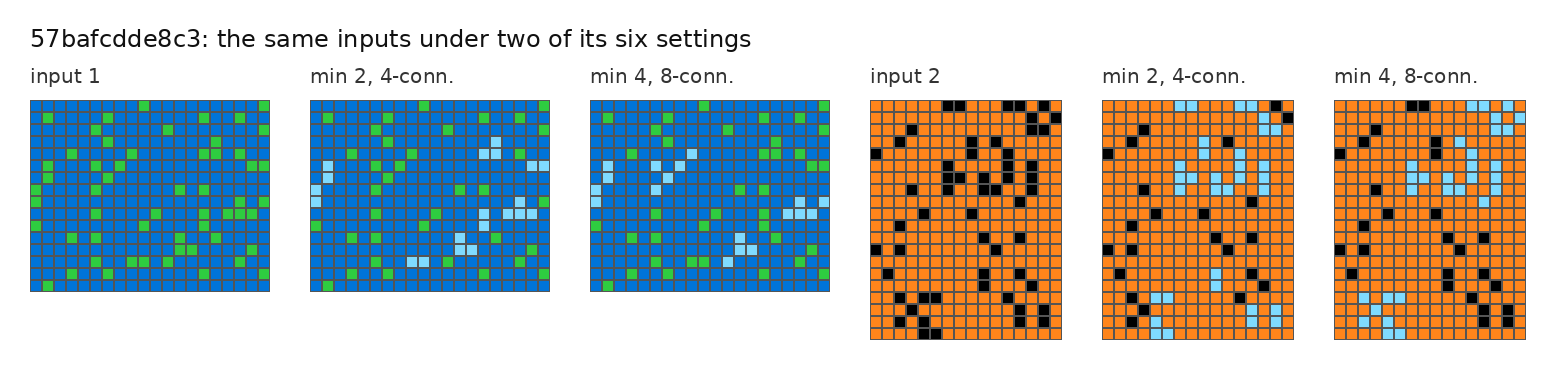
\includegraphics[width=\linewidth]{fig-cherry-57bafcdde8c3.png}
\caption{\gen{57bafcdde8c3}: two demonstration inputs and their outputs under
two of the family's six settings. Larger minimum size and wider connectivity
change which components turn cyan.}
\label{fig:cherry57}
\end{figure}

\begin{figure}[H]
\centering
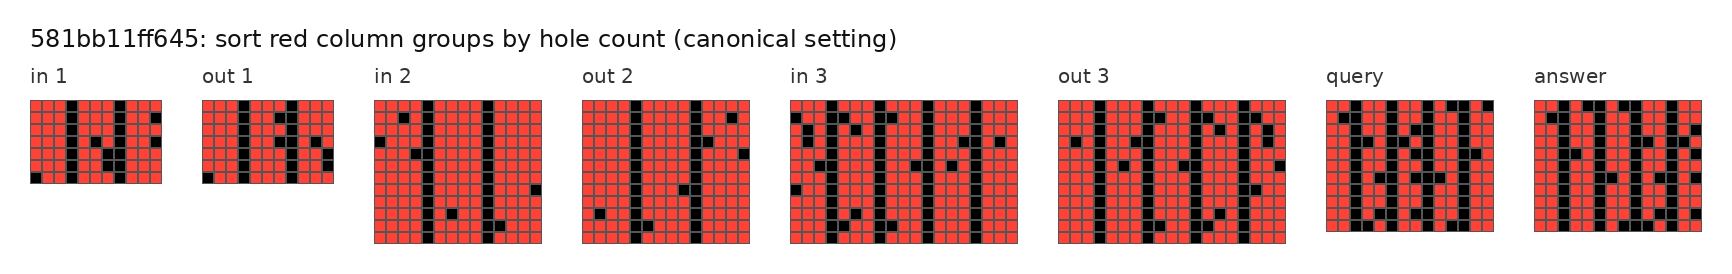
\includegraphics[width=\linewidth]{fig-cherry-581bb11ff645.png}
\caption{\gen{581bb11ff645}: three demonstrations and a query, canonical
setting.}
\label{fig:cherry581}
\end{figure}

\begin{figure}[H]
\centering
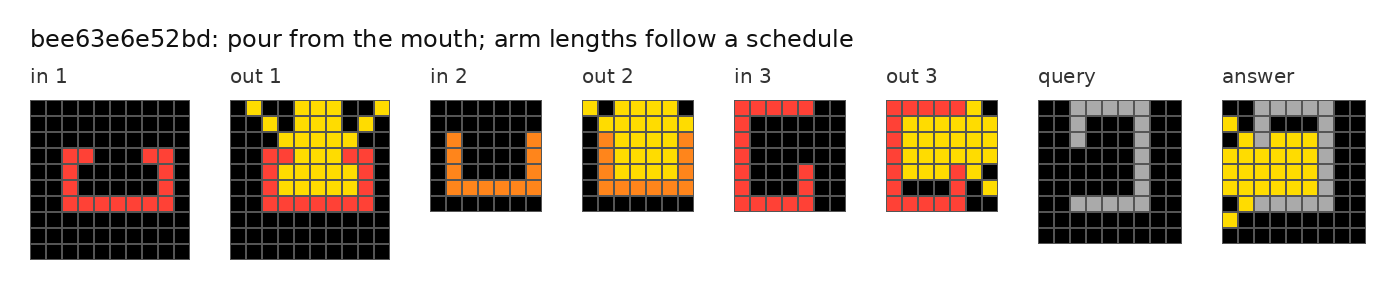
\includegraphics[width=\linewidth]{fig-cherry-bee63e6e52bd.png}
\caption{\gen{bee63e6e52bd}: one lesson (seed 17, sample indices 0--3) with
arm lengths 2/2, 1/1, 1/3 and 3/1.}
\label{fig:cherrybee}
\end{figure}

\paragraph{Drawn at random.} Figure~\ref{fig:random6} shows two
demonstrations from each of six generators drawn uniformly from the 1,984
approved ones (seed 20261108). Section~\ref{sec:reach} measures how many
distinct instances each can produce and what lesson structure each has. Appendix~\ref{app:mastery} shows generators the trained
model found hard, from ARCpuzzles and from RE-ARC, ARC-GEN and NVARC.

\begin{figure}[tbp]
\centering
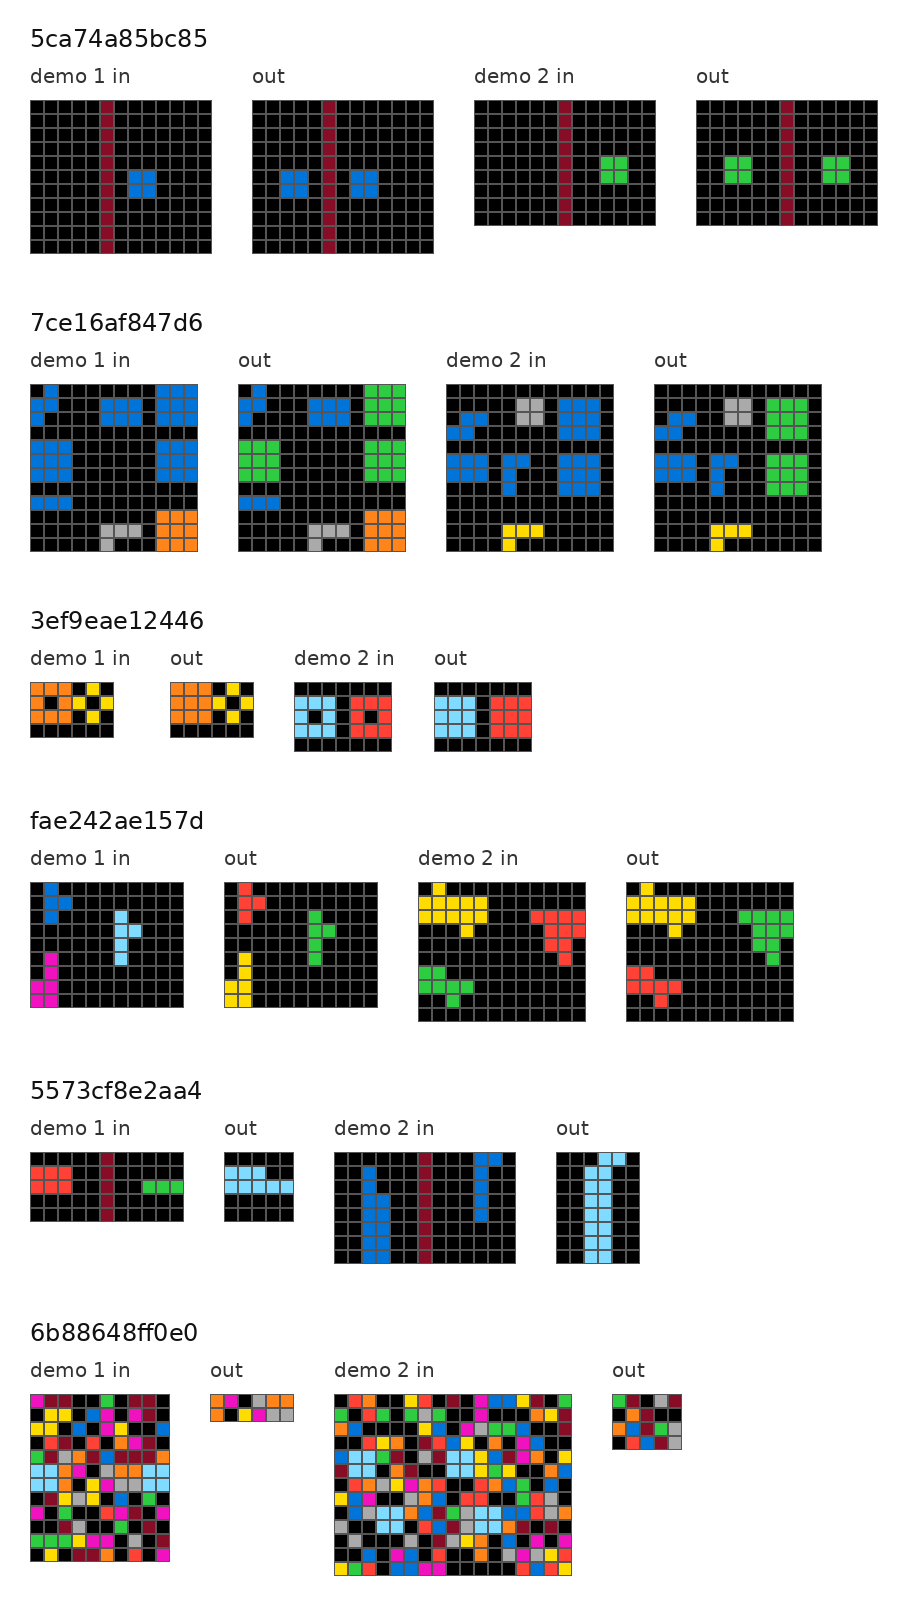
\includegraphics[width=0.75\linewidth]{fig-random-approved-s20261108.png}
\caption{Two demonstrations from each of the six randomly drawn approved
generators.}
\label{fig:random6}
\end{figure}

\section{How the data was made}
\label{sec:made}

\begin{table}[H]
\centering
\begin{tabular}{lr}
\toprule
Source & Generators \\
\midrule
ARC-AGI-2 training tasks & 1,000 \\
ARC-AGI-2 public evaluation tasks & 120 \\
Puzzle bank (Claude and GPT Pro, author-seeded) & 2,859 \\
Custom & 30 \\
Untagged (49 generic concept generators, 3 per-puzzle) & 52 \\
\midrule
Total & 4,061 \\
\bottomrule
\end{tabular}
\caption{Generator sources.}
\label{tab:sources}
\end{table}

\begin{table}[H]
\centering
\small
\begin{tabularx}{\linewidth}{lX}
\toprule
Date (2026) & Milestone \\
\midrule
26 March & Project starts, the day after ARC Prize 2026 opens; an S-expression rule language with parser, evaluator and builtins \\
27 March & Canonical prelude transforms; first grounded traces \\
16 April & First puzzle banks ingested (21-puzzle bundles; 1,785 puzzles that day) \\
27 April & First per-puzzle generators \\
10 May & v0.1 released publicly: 3,889 puzzles, combinatorial axes, helpful and degenerate textures \\
2 July & Defect linter v2: coverage anchored on the original task, axis honesty, mutation testing \\
16 July -- 16 August & Library-wide review of 3,937 generator modules; 693 completed reviews \\
24 July & Semantic gate contract frozen \\
10 September & Library extracted into the independent ARCpuzzles repository \\
3 -- 26 October & Reviewer packets; 1,654 approval receipts \\
22 October -- 2 November & Submission training run, 48 rounds \\
\bottomrule
\end{tabularx}
\caption{Timeline. The two repositories hold about 3,500 commits (2,949 in the
predecessor, 540 in ARCpuzzles).}
\end{table}

Every generator follows the same path:
\begin{enumerate}[nosep]
  \item \textbf{Rule.} A reference rule is written in a constrained Racket DSL. It is the only source of output labels.
  \item \textbf{Generator.} A Python sampler is written against a shared runtime. It states the rule, its sampling axes and its invariants, and optionally declares textures that teach or hide the rule, rival rules and a lesson check.
  \item \textbf{Battery.} Twelve automatic checks run on the generator and rule together.
  \item \textbf{Review.} A reviewer receives a packet for the generator, attacks it, repairs or extends it, and returns the change with evidence.
  \item \textbf{Approval.} An accepted review is recorded against the exact generator and rule hashes. Any later edit revokes approval.
  \item \textbf{Export.} Only approved generators are sampled for training, with answers kept apart from the model-visible challenges.
\end{enumerate}
Puzzle banks were written outside the repository by Claude and GPT Pro, the
models available at the time, seeded with the author's own puzzle ideas. They
came as 21-puzzle bundles (7 easy, 7 medium, 7 hard, each with four training
pairs, a test pair, a written solution and a verified Python solver), were
imported from 16 April, and their solvers were later converted to Racket. The
first generators were written the same way. Later generators were written and
repaired by coding agents under the author's direction; the July review records
Codex, Kimi and OpenAI models as reviewers, and the October reviews were done
by Claude and GPT Pro (Section~\ref{sec:review}).

\section{What a generator does}
\label{sec:generator}

A generator draws fresh tasks for one ARC rule, as many as its input space
allows; for the six measured in Section~\ref{sec:reach} it ranges from 2,376
grids to billions. It has
two halves. A Python sampler,
\texttt{generate(seed, sample\_index, difficulty, **overrides)}, returns one
input grid. A Racket reference rule computes the output. The sampler never
writes outputs.

Most puzzles are identified by a 12-character content hash, a SHA-256 prefix
over their train and test pairs; 172 identifiers, 121 of them approved, use
other forms such as \texttt{public\_eval\_} names. Each generator lives in a
directory named by its identifier. Augmented variants that exercise the same rule share their parent's
identifier and generator.

\texttt{arcpuzzles generate} draws inputs at successive sample indices, drops any
that fail the generator's \texttt{self\_check}, labels the rest with the Racket
rule, and assembles demonstrations and held-out queries into an episode. Each
episode records the executed rule hash, the hash of every input, and the result
of its lesson check.

Generator \gen{0005ab5b7704} (``Marked Column Compression'') keeps the columns
whose row-0 header is yellow. Its complete reference rule:

\begin{lstlisting}[language=Racket]
(rule!
 ;; Keep only the COLUMNS whose header (row 0) is yellow(4); header dropped.
 (let ((keep (filter (lambda (c) (= (at g 0 c) 4)) (range 0 w))))
   (for/list ((r (in-range 1 h)))
     (for/list ((c (in-list keep))) (at g r c)))))
\end{lstlisting}

\begin{figure}[H]
\centering
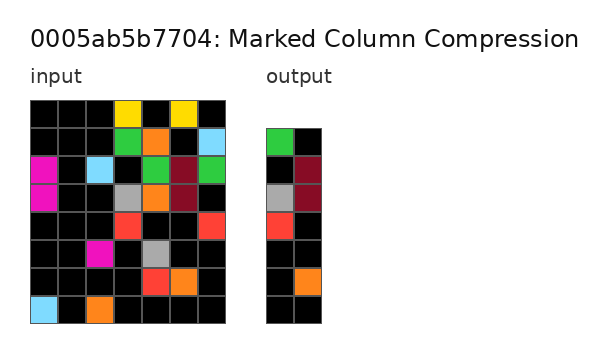
\includegraphics[width=0.45\linewidth]{fig-0005ab5b7704-demo.png}
\caption{A demonstration generated by \gen{0005ab5b7704} (seed 17). Output rows
are drawn level with the input rows they come from.}
\label{fig:0005}
\end{figure}

\paragraph{Why Racket.} We chose Racket for three reasons. It hosts a
domain-specific language naturally: the prelude's grid primitives
(\texttt{objects}, \texttt{recolor-cells}, \texttt{connected-region}, \dots) are
ordinary definitions, so a rule reads in the vocabulary of the task rather than
of a host language. Its prefix notation makes every rule a uniform tree, an
operator followed by its arguments, which is simple to parse, to constrain with
a grammar during decoding, and to lint structurally. And it comes with a REPL, so
a rule can be built and tested one expression at a time against the
demonstrations, by a person or by an agent. The intent was a model that solves tasks the same way, by
writing and running Racket in the REPL. The submission did not train that: it
answers with the grid directly, and the Racket rules served as the source of
every label. The closest it came was the reverse direction: in rounds 7 and 8,
1,440 training examples showed the model a generator's executed Racket rule instead of
demonstrations and trained it to write the output grid for each input
(Appendix~\ref{app:supervision}). It learned to read and execute Racket rules,
never to write them.

\paragraph{Rules are written to one standard.} A written guide (eight chapters,
about 2,100 lines) covers the execution model, a function reference, style,
idioms, gotchas, worked examples, the prelude inventory, and 18 task archetypes
that map what the pairs show (``only colours change'', ``a legend row controls
the behaviour'', ``a template stamps at marker positions'') to a plan and the
prelude functions to use. Its premise is that the rules are themselves training
data for program synthesis, so consistency is quality: each conceptual step is a
named \texttt{define}, the rule ends in one final expression, state is threaded
through folds rather than mutated, and a hand-rolled search where a prelude
function exists is a review defect. A grammar gate checks that the constrained
decoding grammar admits every gold program; it currently fails across the
library, because some rules use primitives the grammar does not list
(Section~\ref{sec:battery}). Once it was clear that the submission would not
train the model to write Racket in time, we stopped holding rules to this
standard: a rule only had to compute the right labels.

\section{Sampling: one shared runtime and keyed draws}
\label{sec:sampling}

All generators share one runtime instead of carrying their own random-number and
grid code.

\subsection{How an instance is drawn}

Fix a generator $G$ with task identifier $t$, version string $v$ and Racket rule
$f$. Write $\sigma$ for an episode seed and $k\in\mathbb{N}$ for a sample index.

\paragraph{Named draws.} Every random choice inside $G$ is a named draw
\texttt{ctx.draw\_*}$(\ell,\dots)$ with a label $\ell$, such as
\texttt{"grid\_h"}. Each label gets its own pseudo-random stream
\[
  R_{\ell}(\sigma,k) \;=\; \mathrm{MT}\!\left(\big\lfloor \mathrm{SHA\text{-}256}(\sigma \,|\, t \,|\, k \,|\, \ell \,|\, v)\big\rfloor_{128}\right),
\]
a Mersenne Twister seeded with the first 128 bits of the digest. A draw's value
therefore depends only on $(\sigma,t,k,\ell,v)$ and its own arguments: adding,
removing or reordering other draws cannot change it. Bare \texttt{random} calls
are forbidden, so an input grid is a deterministic function
\[
  x \;=\; G(\sigma,k).
\]
A caller may override a label; the override replaces $R_\ell$ and must satisfy the
same bounds. Grid size in \gen{0005ab5b7704}:

\begin{lstlisting}[language=Python]
def _dims(ctx, difficulty):
    if difficulty == "easy":
        return ctx.draw_int("grid_h", 6, 8), ctx.draw_int("grid_w", 6, 9)
    if difficulty == "hard":
        return ctx.draw_int("grid_h", 9, 14), ctx.draw_int("grid_w", 11, 16)
    return ctx.draw_int("grid_h", 7, 10), ctx.draw_int("grid_w", 8, 12)
\end{lstlisting}

\paragraph{Episodes.} An episode with $n$ demonstrations and $m$ queries tries
sample indices $k_0, k_0+1, \dots$ in order. Index $k$ is accepted when $x_k =
G(\sigma,k)$ is a well-formed grid, $G$'s \texttt{self\_check} returns no
findings and leaves $x_k$ unchanged, $y_k = f(x_k)$ executes, $y_k \neq x_k$
unless the task allows identity outputs, and $(x_k,y_k)$ is not a repeat. With
$k_1<\dots<k_{n+m}$ the first $n+m$ accepted indices in $[k_0,\,k_0+5(n+m))$, the
demonstrations are $(x_{k_i}, f(x_{k_i}))_{i\le n}$ and the queries are the rest.
Fewer acceptances fail the episode; every rejected index is logged with its
reason.

\paragraph{Exports.} An export with seed $s$ over a pool $P$ with mix weights
$w$ uses one generator $r=\mathrm{MT}(s)$. Attempt $j$ draws a generator
$g_j$ with $\Pr(g_j=g)=w_g/\sum_{h\in P}w_h$ (or uniformly), then an episode seed
$\sigma_j$ of 63 bits, both from $r$. The same sequence drives planning and
execution, including rejected attempts, so an export is reproducible from
$(s,P,w)$. The \texttt{generate} command uses $\sigma_i = s+i$ for episode $i$.
A parametric export also uses $\sigma_i=s+i$ and draws the rule setting
$\theta_i$ uniformly from the family's settings $\Theta$ with $\mathrm{MT}(s+i)$;
every pair of the episode uses $f_{\theta_i}$.

\paragraph{Overrides.} Any named axis can be pinned by the caller, and the pinned
value passes the same validity check as a random one. The override checker probes
every declared axis at its boundaries and in combination, and generators declare
which combinations they legitimately refuse.

\paragraph{Axis honesty.} Each draw records the bounds it actually used. The
defect linter compares those bounds with the declared axes, so a generator cannot
claim a range it never samples.

\paragraph{Difficulty.} \texttt{easy}, \texttt{medium} and \texttt{hard} select
bands within each axis, so a curriculum changes scale without changing the rule.

\paragraph{Shared helpers.} Grid, placement, palette, object, shape, panel, room,
lattice and texture helpers are shared, so a fix to a placement bug reaches every
generator that uses it. The rule runtime also provides 18 rule templates, composable
factories for common rule shapes (recolour map, colour swap, recolour by size,
fill enclosed regions, gravity, mirror, symmetry completion, upscale, tile,
per-object transforms, keep or remove a colour, crop to an object, sort objects,
connect dots, extend lines), callable as \texttt{template!} in the rule REPL.

\paragraph{Rejections.} The runner records every rejected pair with a
phase-prefixed reason, and drops duplicate and identity pairs.

\subsection{Lessons, not samples}

The sample index is not only a source of randomness. In most generators it is a
position in a lesson schedule: a function $\pi:\mathbb{N}\to\mathcal{P}$ onto a
small set of scene profiles, usually $\pi(k)=\mathcal{P}_{k \bmod p}$, chosen
so that every window of consecutive indices contains inputs that refute the
rivals of Section~\ref{sec:rivals}. The seed then varies the surface (colours,
positions, shapes, counts) inside each profile. Because an episode takes accepted indices in order from $k_0$, a schedule of
period $p$ places every profile in any lesson of at least $p$ pairs whose indices
are consecutive, that is, when no draw inside the window was rejected. Of the 1,984 approved generators, 1,007 declare such a schedule.

\subsection{Reach and expressiveness: six approved generators drawn at random}
\label{sec:reach}

The set of grids a generator can emit is its image
$\mathrm{Im}(G)=\{G(\sigma,k)\}$, and its draw distribution is $p(x)=\Pr[G(\sigma,k)=x]$.
We report three quantities.
\begin{itemize}[nosep]
  \item $S_{\mathrm{obs}}$: distinct inputs among $N$ draws $(\sigma,k)=(j,j)$, $j<N$; a lower bound on $|\mathrm{Im}(G)|$.
  \item Chao1, $\hat S = S_{\mathrm{obs}} + f_1^2/(2f_2)$, where $f_1,f_2$ count grids seen once and twice: a lower-bound estimator of $|\mathrm{Im}(G)|$.
  \item The effective size $N_{\mathrm{eff}} = 1/\sum_x p(x)^2$, the number of equally likely grids with the same collision rate. It satisfies $N_{\mathrm{eff}} \le |\mathrm{Im}(G)|$, with equality for uniform $p$. Since $2C/(N(N-1))$ is an unbiased estimate of $\sum_x p(x)^2$, where $C$ is the number of colliding pairs among the $N$ draws, we report $\hat N_{\mathrm{eff}} = N(N-1)/(2C)$.
\end{itemize}

We drew six generators uniformly from the 1,984 approved ones (seed 20261108).
None was chosen by hand.

\paragraph{An exact case.} \gen{3ef9eae12446} (fill the zero centre of a
$3\times3$ ring whose eight border cells share one colour) can be counted
directly. Without a difficulty band, $k \bmod 6$ fixes both the grid size $(h,w)
\in \{(4,6),(5,7),(6,7),(5,8),(4,7),(6,8)\}$ and the profile. The seed chooses
an ordered colour pair ($9\cdot8=72$ ways), the motif row ($h-2$ ways) and which
end holds the target (2 ways). The \texttt{multi\_target} phase paints two rings
and is symmetric under swapping both colours and ends. Hence
\[
  |\mathrm{Im}(G)| \;=\; \sum_{\text{phases}} 2\cdot72\,(h-2) \;-\; \tfrac12\cdot 2\cdot72\cdot3 \;=\; 2{,}592 - 216 \;=\; 2{,}376,
\]
and, with the six phases equally likely and grids uniform within a phase,
$N_{\mathrm{eff}} = 2{,}073.6$ exactly. From $N=20{,}000$ draws we measure
$S_{\mathrm{obs}}=2{,}374$, Chao1 $=2{,}378$ and $N_{\mathrm{eff}}\approx2{,}075$,
which validates the estimators.

\begin{table}[H]
\centering
\small
\begin{tabular}{lrrrrrrr}
\toprule
Generator & Declared & $|\Theta|$ & $N$ & $S_{\mathrm{obs}}$ & Chao1 & $N_{\mathrm{eff}}$ & Grid shapes \\
\midrule
\gen{3ef9eae12446} & 196 & 1 & 20k & 2,374 & 2,378 & 2,075 & 6 \\
\gen{5ca74a85bc85} & 16 & 1 & 20k & 13,349 & 62,000$^{\uparrow}$ & 146 & 24 \\
\gen{5573cf8e2aa4} & 150 & 1 & 20k & 14,837 & 365,000$^{\uparrow}$ & 14,000 & 25 \\
\gen{7ce16af847d6} & 3 & 2 & 100k & 99,997 & -- & $\approx1.7\times10^{9}$ & 2 \\
\gen{fae242ae157d} & 54 & 3 & 100k & 99,998 & -- & $\approx2.5\times10^{9}$ & 6 \\
\gen{6b88648ff0e0} & 14 & 3 & 100k & 100,000 & -- & $\gtrsim1.7\times10^{9}$ & 165 \\
\bottomrule
\end{tabular}
\caption{Declared configurations ($\prod_j|A_j|$), rule settings, and measured
reach. Grid shapes are counted over 5,000 draws. Chao1 values marked
$^{\uparrow}$ were still rising with $N$; they are estimates at the stated $N$,
not bounds. ``--'': too few repeats for Chao1. For
\gen{6b88648ff0e0} no collision occurred; the bound uses $C\le3$, the 95\%
upper limit for zero observed events.}
\end{table}

Declared configurations and measured reach disagree in both directions.
\gen{7ce16af847d6} declares three configurations and produced 99,997 distinct
grids in 100,000 draws; \gen{3ef9eae12446} declares 196 and emits exactly
2,376. The declared axes list the structural choices a generator makes;
everything else, such as colours, positions and shapes, varies with the seed.

\begin{table}[H]
\centering
\small
\begin{tabularx}{\linewidth}{lXlXr}
\toprule
Generator & Rule & Schedule $\pi$ & Rivals (fit the original pairs) & Amb. \\
\midrule
\gen{3ef9eae12446} & fill centre of a uniform $3\times3$ ring & $k \bmod 6$ & 1 (1): four-neighbour-only test & 0 \\
\gen{7ce16af847d6} & recolour exact solid blue $3\times3$ components & $(\sigma+k)\bmod 3$ & 5 (3): bbox-only, size-only, contains-window, any colour, all blue & 0 \\
\gen{fae242ae157d} & recolour three objects 2/3/4 by area rank & $k \bmod 3$, $k \bmod 6$ & 6 (3): scan order, fixed areas 4/5/6, scene position, colour rank, descending, identity & 0 \\
\gen{5573cf8e2aa4} & union of two panels' occupancy & anchor at $k\equiv0 \pmod 3$ & 5 (1): intersection, XOR, copy left, copy right, cell inequality & 0 \\
\gen{5ca74a85bc85} & mirror source cells across a divider & none; 5 replay, 11 general profiles & 1 (1): filled source bounding box & 4 \\
\gen{6b88648ff0e0} & stack strips between cyan markers & none & 0 in production; family audit of 26 policies & -- \\
\bottomrule
\end{tabularx}
\caption{Lesson structure of the six sampled generators. In parentheses: rivals
that reproduce every labelled original pair, measured by
\texttt{arcpuzzles lesson-census}. Amb.: of 60 census lessons (20 per difficulty
band, 3 demonstrations and 1 query, explicit demonstration count), those in which
a declared rival fits every demonstration but changes the query answer.}
\end{table}

\paragraph{What the six show.}
\begin{itemize}[nosep]
  \item \textbf{The original demonstrations are often under-determined.} In five of the six, at least one simple rival fits every labelled original pair. For \gen{5573cf8e2aa4} it is raw cell inequality (mark a cell where the two panels differ): each original pair gives its two panels different colours, so an occupied overlap is unequal and is marked exactly as union marks it. Ordinary draws of the generator give both panels one shared colour, which separates the two rules. Because these rivals reproduce the test pairs too, they score perfectly on the original task: the ambiguity is invisible to the task's own score, but data that only imitates the original inputs would teach the shortcut as readily as the rule. For \gen{fae242ae157d}, every official example uses areas 4/5/6 in ascending scan order, so ``rank by area'', ``rank by scan order'' and ``map 4/5/6 to 2/3/4'' agree on all of them.
  \item \textbf{Schedules are designed against query rotation.} The six-slot schedule of \gen{3ef9eae12446} places the cornerless-cross witness at three positions so that every cyclic window of four pairs keeps one among its demonstrations, whichever pair is held out as the query. A four-slot schedule was rejected because it could hold out the only witness.
  \item \textbf{Replay anchors trade effective size for coverage of the original.} \gen{5ca74a85bc85} draws its five public profiles with weight 1 and its eleven general profiles with weight 2, so $5/27\approx18.5\%$ of draws replay an original input exactly. This concentrates mass ($N_{\mathrm{eff}}=146$) while the general profiles keep the image large (Chao1 $\ge 62{,}000$ and rising).
  \item \textbf{Honest axes replaced advertised ones.} The imported version of \gen{7ce16af847d6} was a fixed five-component fixture that advertised nine controls; the imported \gen{5573cf8e2aa4} declared nine axes, several singleton, aliased or inert. Both rewrites expose only exact, observable axes. Declared reach fell; measured reach rose.
  \item \textbf{Census lessons refute the declared rivals, with one exception.} Four of the five generators that declare rivals produced no ambiguous lesson in 60. \gen{5ca74a85bc85}, which has no schedule, produced 4: the filled-bounding-box rival fits all three demonstrations and changes the query answer. In 21 more its demonstrations do not refute the rival, but the rival gives the right query answer. When export chooses the demonstration count, the worker rejects an ambiguous lesson. When the caller fixes the count, as the census does, the lesson is kept and its provenance records \texttt{diagnostic\_unsupported}.
  \item \textbf{A declaration can be wrong, and approval does not follow a stricter gate.} The generator \gen{5573cf8e2aa4} sets \texttt{CANONICAL\_SHORTCUTS} to a copy of \texttt{LESSON\_COMPETITORS}, declaring all five rivals to fit the original pairs. On 23 October the semantic gate began checking each declared shortcut against the labelled original pairs; intersection, copy-left and copy-right fit none of the three, and XOR fits one. The generator was approved on 3 October, has not changed since, and fails today's gate. Its lessons are not affected (no ambiguous census lesson; every witness fires), but the label ``canonical shortcut'' is wrong for four of its rivals. 356 approved generators copy their whole rival list into \texttt{CANONICAL\_SHORTCUTS} this way. Of five drawn from them at random (seed 20261108), two fail today's gate for the same reason (\gen{6d26bc40cbb2}, three shortcuts; \gen{99e7ba062bec}, five) and three pass.
  \item \textbf{The trained model mastered three of the six and found two more easy.} Measured by prefill scans of fresh draws (Appendix~\ref{app:mastery}), \gen{3ef9eae12446}, \gen{5573cf8e2aa4} and \gen{5ca74a85bc85} were mastered by the end of the run, \gen{7ce16af847d6} and \gen{6b88648ff0e0} were easy, and \gen{fae242ae157d}, the generator with the most rivals, was medium: 21\% of its scanned draws mastered and 25 of 40 greedy answers right.
\end{itemize}



\section{Textures: making the rule visible}
\label{sec:textures}

A texture is a named kind of input a generator can draw, such as sparse
objects, stripes or a full grid. A generator can declare \emph{helpful}
textures, which make the rule visible, and \emph{degenerate} textures, which
hide it. Degenerate textures are reachable only by explicit override, never on
the default path, and the self-check stage fails a generator if one leaks into
ordinary output. Declaring textures is optional: of the 1,984 approved
generators, 264 name helpful textures and 255 name degenerate ones (459
distinct names). Counting texture sampling axes and lawful degenerate
textures as well, 347 declare textures in some form. Across the whole library, 1,881
generators name degenerate textures.

\begin{table}[H]
\centering
\begin{tabularx}{\linewidth}{XX}
\toprule
Helpful (examples) & Degenerate (generators declaring it) \\
\midrule
noise, sparse, blob, stripes, gradient & \texttt{full\_grid} (356) \\
checkerboard, frame, ring, plus & \texttt{no\_markers} (101), \texttt{no\_seeds} (77) \\
task-specific palettes: warm, cool, varied & \texttt{no\_pairs} (73), \texttt{no\_blobs} (73), \texttt{no\_objects} (69) \\
 & \texttt{single\_motif} (53), \texttt{all\_same\_color} (52), \texttt{monochrome} (38) \\
\bottomrule
\end{tabularx}
\caption{Texture examples across the whole library, approved or not. 1,962
distinct degenerate texture names are declared.}
\end{table}

In \gen{0005ab5b7704}, the invariants require content in both kept and dropped
columns, so keep-versus-drop shows in every output. Its degenerate textures are
\texttt{no\_markers}, \texttt{all\_columns\_marked} and \texttt{no\_body}.

\begin{figure}[H]
\centering
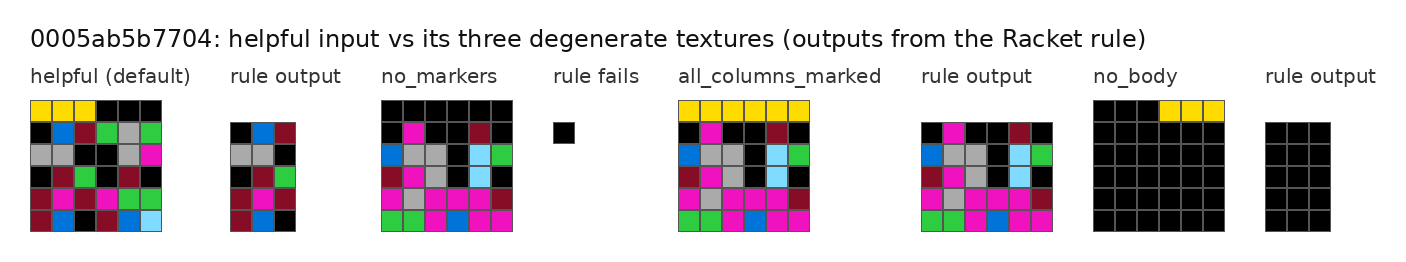
\includegraphics[width=\linewidth]{fig-textures-0005ab5b7704.png}
\caption{A helpful input of \gen{0005ab5b7704} and its three degenerate
textures, labelled by the Racket rule. With no markers the rule has no column
to keep and fails (shown as a single black cell); with every column marked the
output is the whole body, so keep-versus-drop is invisible; with no body every
output cell is black. The generator's \texttt{self\_check} rejects all three:
``row 0 has no color-4 markers'', ``every column is marked'', and ``no selected
column has a nonzero body cell''.}
\end{figure}

\section{Rival rules: attacking the rule}
\label{sec:rivals}

A generator can declare rival rules: plausible alternatives a solver might infer
instead of the real one. The semantic gate checks that generated lessons
eliminate them.
\begin{itemize}[nosep]
  \item \texttt{SEMANTIC\_RIVALS}: named alternative rules, each a function from grid to grid.
  \item \texttt{SEMANTIC\_WITNESSES}, \texttt{WITNESS\_RIVALS}: input features, each tied to the rivals it must refute. Whenever an input has a witness feature, at least one of the rivals tied to it must give a different output from the reference rule on that input.
  \item \texttt{lesson\_identifiable}: rejects a lesson in which a rival fits every demonstration but changes the query answer, when export chooses the demonstration count; with a fixed count the lesson is kept and flagged.
  \item \texttt{CANONICAL\_SHORTCUTS}: rivals that also fit the original ARC task's own pairs. Each needs generated counterexamples. Since 23 October the gate also verifies the fit and fails a declared shortcut that misses any labelled original pair; generators approved earlier were not re-gated (Section~\ref{sec:reach}).
\end{itemize}

1,498 generators declare 6,822 rivals, a median of 4 and up to 25 per generator,
under 5,085 distinct names. Among the 1,984 approved generators, 1,352 declare rivals, 1,224 a
lesson-identifiability check and at least 761 canonical shortcuts (1,223 by a looser text match). Most rivals are written for one task. The most common
are \texttt{identity} (175 generators), \texttt{horizontal\_only} (42),
\texttt{vertical\_only} (38), \texttt{solid\_bbox} (19),
\texttt{largest\_component\_only} (15) and \texttt{ignore\_blockers} (14).

Generator \gen{00ed2544a15e} fills the cells between two red cells with cyan when
the segment between them holds nothing else. Two of its rivals reproduce every
pair in the original ARC task:

\begin{lstlisting}[language=Python]
def _rival_ignore_blockers(grid):
    """Connect every exactly-two-red aligned span, ignoring other colors.

    Every interior cell is painted, including a blocker. This reproduces every
    canonical example because none places a distractor inside a red-red span,
    but it disagrees on every generated blocked pair.
    """
\end{lstlisting}

\texttt{simple\_pairs\_only}, which connects only isolated pairs, also fits all
original demonstrations because they contain only disjoint pairs. The original
task does not separate these rules from the intended one. The generator does:
every ordinary example contains a horizontal and a vertical connection, a pair
blocked by another colour, an isolated red, and a chain or shared endpoint
(Figure~\ref{fig:00ed}).

\begin{figure}[H]
\centering
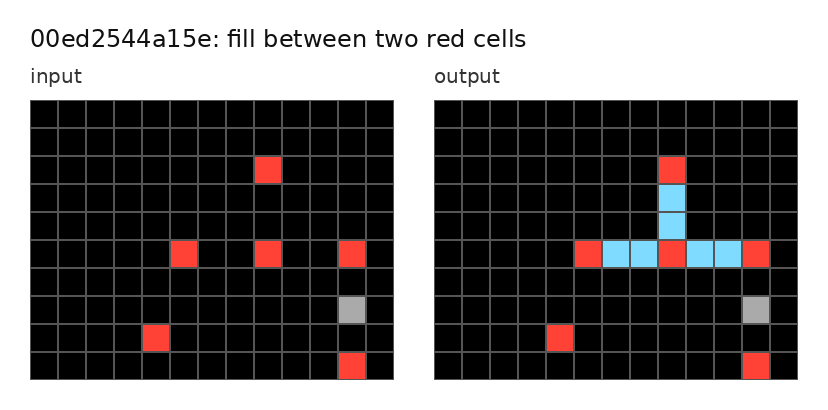
\includegraphics[width=0.7\linewidth]{fig-00ed2544a15e-demo.png}
\caption{A demonstration generated by \gen{00ed2544a15e} (seed 17): a chain of
three reds with a shared endpoint, a vertical connection, a pair blocked by grey
(left unfilled), and an isolated red.}
\label{fig:00ed}
\end{figure}

\begin{table}[H]
\centering
\begin{tabular}{ll}
\toprule
Rival rule & Result on the seed-17 lesson \\
\midrule
identity & refuted \\
horizontal pairs only & refuted \\
vertical pairs only & refuted \\
ignore blocking colours (fits the original task) & refuted \\
simple pairs only (fits the original task) & refuted \\
\bottomrule
\end{tabular}
\caption{Lesson check recorded in a generated \gen{00ed2544a15e} episode with
three demonstrations. A full semantic-gate run on this generator passed on
8~November 2026.}
\end{table}

These checks are sampled evidence against named alternatives, not proof that no
other rule fits the demonstrations.

\section{Templates: parametric Racket rules}
\label{sec:parametric}

941 generators have an accepted parametric family: one input sampler shared by
several rule settings, each with its own Racket program. All pairs in an episode
use one setting, and the demonstrations must tell the settings apart. The
family's declared shortcuts are checked when the family is accepted. Every
episode is certified when it is drawn, against the family's settings:
each setting's program runs in Racket on the demonstrations, the drawn setting
must be the only one that reproduces them all, and every query label must agree
among the survivors; otherwise the episode is rejected. The 941 families have 2,174 settings, each with its own Racket
program (2,170 distinct program hashes). In every family the default setting is
byte-for-byte the canonical program, so the families add 1,233 rule variants to
the library. Most families have one parameter with two settings (759); 29 have
two or three parameters, with up to 12 settings.

\gen{0005ab5b7704} adds a setting that orders the selected columns by how many
non-black body cells they hold:

\begin{lstlisting}[language=Racket]
(rule!
 ;; Stage A selects only header-marked columns and measures their body occupancy.
 (let ((keep (filter (lambda (c) (= (at g 0 c) 4)) (range 0 w))))
   (define (body-count c)
     (length (filter (lambda (r) (not (= (at g r c) 0))) (range 1 h))))
   ;; Stage B orders that selected-and-measured intermediate, then packs the body.
   (let ((ordered (sort keep (lambda (a b)
                               (let ((ca (body-count a)) (cb (body-count b)))
                                 (or (> ca cb) (and (= ca cb) (< a b))))))))
     (for/list ((r (in-range 1 h)))
       (for/list ((c (in-list ordered))) (at g r c))))))
\end{lstlisting}

The family keeps an adversarial rule, \texttt{wrong\_intermediate.rkt}, that
counts the marked columns and then keeps that many of the densest columns in
the whole grid, marked or not. To refute it, the sampler
gives the marked columns distinct densities, forces an order that differs from
left to right, and always includes a dense unmarked column. A 32-seed audit and a
256-seed sweep found no surviving declared shortcut. In the exported episode of
Figure~\ref{fig:param}, unmarked column 1 holds seven body cells and outranks the
marked columns under the adversarial rule; all three demonstrations of that
episode refute it.

\begin{figure}[H]
\centering
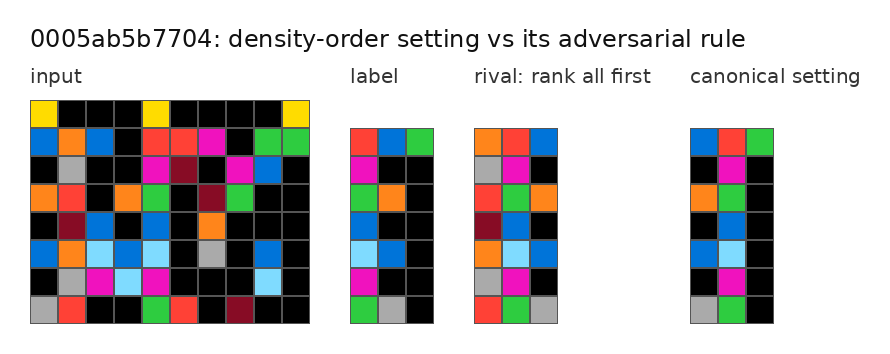
\includegraphics[width=0.85\linewidth]{fig-0005ab5b7704-parametric.png}
\caption{One demonstration from an exported \texttt{body\_density\_desc} episode
(seed 12). From left: input; Racket label; the adversarial rule's answer; the
canonical setting's answer.}
\label{fig:param}
\end{figure}

\begin{table}[H]
\centering
\begin{tabularx}{\linewidth}{lXX}
\toprule
Family & Settings & Lesson requirement \\
\midrule
\gen{57bafcdde8c3} & minimum size 2, 3, 4 $\times$ connectivity 4, 8 & Separate all six settings and five shortcuts; queries up to 30$\times$30 \\
\gen{7b0cb3b9a618} & front or back crossing band & Reject eight declared shortcuts under both settings \\
\gen{581bb11ff645} & count cells or regions $\times$ ascending or descending & The first demonstration separates every setting \\
\gen{0005ab5b7704} & left to right or by density & Refute ranking all columns before selection \\
\bottomrule
\end{tabularx}
\caption{Representative accepted parametric families.}
\end{table}

\section{Matching the original task}
\label{sec:matching}

Generated inputs must cover the task they imitate. A distribution gate compares
object count, component size, palette size and area with the original
demonstrations. A profile floor fails a generator if no generated grid matches
any original (height, width, palette) profile, or if its \texttt{self\_check}
rejects an original input.

\section{The check battery}
\label{sec:battery}

Labels are correct by construction once the rule runs as reviewed;
\texttt{rule\_smoke}, \texttt{authority\_sync} and \texttt{selfcheck} protect
that construction. Most other stages, like the rival rules, are regularizers on
the data: they push a generator toward lessons a learner can use. A few judge
how a Racket rule is written rather than what it computes.
\texttt{racket\_lint} enforces the house style, for example
\texttt{(at g r c)} rather than \texttt{(cell-at g r c)}; nine of its thirteen
checks are style or size rules. \texttt{grammar} asks whether the constrained
decoding grammar admits every gold program, and \texttt{authority\_sync} also
fails when two copies of a rule differ only in text. These matter only if the
rules themselves become training data for writing programs. Once the
submission could not train that in time, we stopped fixing such findings, and
reviewer requests aimed at them were left open: a helper to synchronize
behaviour-identical rule copies, a wider grammar, and fewer false alarms from
the lint that flags Python names matching Racket primitives. The labels do not
depend on them. The twelve
stages cover structure (\texttt{lint}, \texttt{override},
\texttt{racket\_lint}, \texttt{grammar}), execution (\texttt{selfcheck},
\texttt{rule\_smoke}), distribution (\texttt{dist\_gate},
\texttt{profile\_floor}, \texttt{diversity}) and semantics
(\texttt{semantic\_\allowbreak gate}, \texttt{defect\_\allowbreak lint}, \texttt{authority\_\allowbreak sync}). Each
began as a defect reviewers found by hand.

\begin{table}[H]
\centering
\begin{tabularx}{\linewidth}{Xl}
\toprule
Defect found in review & Check that now catches it \\
\midrule
Generated median object count 12 against the original's 2 & \texttt{dist\_gate} \\
0\% of generated grids match any original grid profile & \texttt{profile\_floor} \\
Passed 120 of 120 execution runs while teaching the wrong key-to-direction mapping & \texttt{semantic\_gate} \\
Ordinary draws that were identity transforms & \texttt{semantic\_gate} \\
Gold program calls a helper the constrained grammar rejects & \texttt{grammar} \\
Generator crashes or emits constant outputs yet passes lint & \texttt{rule\_smoke}, \texttt{selfcheck} \\
\bottomrule
\end{tabularx}
\caption{Defects that produced checks.}
\end{table}

\paragraph{Today's battery on the six sampled generators.} The battery keeps
growing, and approval is not re-run when it does. We ran today's twelve stages
on the six generators of Section~\ref{sec:reach}; none passes all twelve. All
six pass \texttt{lint}, \texttt{selfcheck}, \texttt{rule\_smoke},
\texttt{dist\_gate}, \texttt{profile\_floor}, \texttt{diversity},
\texttt{override} and \texttt{racket\_lint}. All six fail \texttt{grammar}, a
library-wide gate that fails because rules elsewhere use primitives the
grammar does not list (\texttt{build-list}, \texttt{string-append},
\dots), and \texttt{defect\_lint}, whose newer \texttt{strict-scalar} detector
finds that the generators accept invalid argument types (a boolean seed, a
negative sample index, an unknown difficulty) instead of rejecting them.
Neither changes the data drawn with valid arguments. Two fail
\texttt{semantic\_gate}: \gen{5573cf8e2aa4} on its shortcut declarations
(Section~\ref{sec:reach}), and \gen{5ca74a85bc85} because 4 of 12 raw lessons
fit its declared rival, which automatic export rejects. \gen{6b88648ff0e0}
fails \texttt{authority\_sync}: its two active copies of the rule differ in
exact text, though they execute identically, and it declares no semantic
contract, so its semantic gate is advisory.

\paragraph{Reviewing the reviewers.} During the July review, an independent
audit replayed reviewers' claims and published each gap as a numbered,
mandatory correction. Every later review had to acknowledge all active items.
\begin{itemize}[nosep]
  \item \textbf{KRF-0001} (16 July): a tier-4 harness rating was not supported
  by a boundary cross-product probe. Overrides must be checked exactly, not
  merely accepted.
  \item \textbf{KRF-0002}: in \gen{f2865c4fa81f}, 519 of 900 accepted
  \texttt{strict\_subset=False} draws silently fell back to subset geometry,
  although the generic replay passed because some draws differed. The override
  contract now checks every accepted request against its observed value.
  \item \textbf{KRF-0003} (17 July): generators that passed every green gate
  still did not represent the task's manifold. This produced the semantic gate,
  whose contract was frozen on 24 July.
  \item \textbf{KRF-0004}: early-return code paths chose dimensions without the
  declared axis labels, escaping the axis-honesty check.
  \item \textbf{KRF-0005}: a healthy aggregate mutation-rejection rate hid one
  degenerate family that \texttt{self\_check} still accepted. Each named impostor
  is now an individual obligation.
\end{itemize}

\section{Review and approval}
\label{sec:review}

Review ran in two phases.

\paragraph{July--August 2026: every generator, one at a time.} A queue covered
all 3,937 generator modules then in the library. Each item had to end in an
improvement or an evidence-backed ``no change'' and a rating on six categories,
each tier 0--4 (poisonous, deficient, adequate, strong, exemplary) with a line
of evidence citing a command, metric or file. The tiers have measurable
thresholds; for example, diversity tier~3 requires at least 90\% distinct
inputs in every difficulty band with independently varying axes, and coverage
tier~3 requires branch counts measured per band, a worst-to-best branch ratio
no worse than 1:10, and an explicit witness for every shortcut hypothesis.
693 reviews were completed, by Codex (255), Kimi (136), OpenAI models (16) and
others. They checked 4,890 shortcut hypotheses (median 7 per generator), each
with witness counts per difficulty band, and 5,355 original pairs.

\begin{table}[H]
\centering
\small
\begin{tabular}{lrrrr}
\toprule
Category & Tier 1 & Tier 2 & Tier 3 & Tier 4 \\
\midrule
Coverage of rule branches & 0 & 2 & 379 & 312 \\
Diversity & 0 & 25 & 433 & 235 \\
Reference rule generality & 0 & 15 & 196 & 482 \\
Harness compliance & 0 & 2 & 80 & 611 \\
Source synchronisation & 3 & 19 & 104 & 567 \\
Training suitability & 4 & 101 & 449 & 139 \\
\bottomrule
\end{tabular}
\caption{Tiers assigned by reviewers after repair, 693 July--August reviews.
Where before-and-after metrics were recorded, defect-lint issues fell from a
median of 4 to 0 (51 reviews) and distinct input/output pairs rose from 64\% to
100\% (12 reviews).}
\end{table}

\paragraph{October 2026: reviewer packets.}

Reviewers, Claude and GPT Pro, receive packets for assigned generators and
return repairs, extensions and evidence, which are integrated against the
source hashes they were assigned. Appendix~\ref{app:packet} quotes their
instructions.
569 integrated review records are retained for 486 generators; older processed
returns were compacted once their content was integrated.

Each packet begins with a blind solve of a separate approved task, before any
reference material is opened; the reviewer writes and revises a Python
\texttt{solve(grid)} against the visible demonstrations, and every revision,
wrong answer and timeout is kept. After the repair, the reviewer solves a fresh
episode of the repaired generator, with its query answers scored privately after
return. Every reviewer also answers a standing question: \emph{name the
strongest plausible rival rule that fits the original demonstrations, give an
exact input on which it disagrees with the intended rule, say how the output
was checked, and say whether the generator now emits such cases.} 629 approved
generators keep a current answer, each with an exact input. For
\gen{bee63e6e52bd}, in which yellow pours from the gap in a frame and continues
diagonally past both arm tips, the answer names \emph{fixed two-cell mouth arms}: every original pair has arms of
length 2 at both ends, so a rule that assumes 2/2 arms reproduces all four
original labels, and a right-open $7\times7$ frame with arms of length 1 and 3
separates it from the intended rule (Figure~\ref{fig:bee6}). The generator now
schedules arms of 1/1, 1/3 and 3/1. The library
retains 2,638 solve attempts across 1,425 generators: 1,283 blind solves before
repair (1,273 with no earlier exposure to the rule) and 1,355 after repair.
By the reviewers' own reports, 2,499 attempts reproduce every visible
demonstration. Maintainers scored the hidden queries of 104 attempts on 91
generators (10 blind, 94 after repair): 96 programs pass both the visible
demonstrations and the hidden queries, 6 fail both, and 2 fail a visible
demonstration yet answer the queries correctly. None reproduces every visible
demonstration and then misses a hidden query, which is what a solver would
produce on a lesson whose demonstrations admit a second rule. The other
attempts are reviewer-reported and unscored.

\begin{figure}[H]
\centering
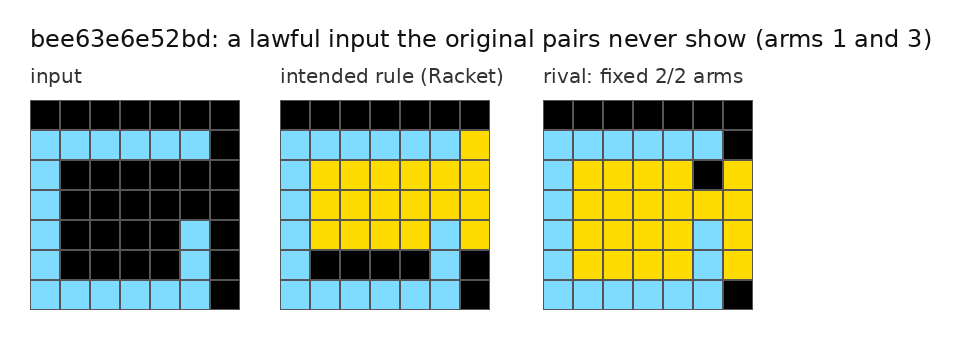
\includegraphics[width=0.85\linewidth]{fig-bee63e6e52bd-shortcut.png}
\caption{A reviewer's answer to the standing question for \gen{bee63e6e52bd},
replayed: the input quoted in the answer, the reference rule's output, and the
output of the declared rival that assumes both arms have length 2. Both rules
reproduce all four original pairs.}
\label{fig:bee6}
\end{figure}

\begin{table}[H]
\centering
\begin{tabular}{lr}
\toprule
Review outcome & Records \\
\midrule
Accepted repair & 201 \\
Accepted new prototype & 291 \\
Needs more evidence & 69 \\
Blocked, deferred or other & 8 \\
\bottomrule
\end{tabular}
\caption{Retained review outcomes. 568 of 569 report reviewer-run results that
were not re-run when integrated.}
\end{table}

Approval requires a \texttt{reviewed\_safe} label recorded against the current
generator and rule hashes; the labels and the full definition are in
Section~\ref{sec:release}. Editing a reviewed generator revokes its approval
until it is reviewed again: 56 generators are unapproved because their code
changed after review, and 15 because their rule did.

\section{Comparison with RE-ARC, ARC-GEN and NVARC}
\label{sec:compare}

Each dataset produces pairs $(x,y)$ and certifies something about them. Stated
precisely:

\begin{description}[nosep,leftmargin=1.5em]
  \item[RE-ARC \cite{rearc}.] A hand-written generator $G_t$ for each of the 400
  ARC-AGI-1 training tasks emits $(x,y)=G_t(\omega)$; the pair is kept iff a
  separately written DSL solver $V_t$ satisfies $V_t(x)=y$. Certified: two
  programs agree on each pair.
  \item[ARC-GEN \cite{arcgen}.] A generator $G_t(\theta)$ emits $(x,y)$ for 400
  ARC-AGI-1 tasks and 500 ARC-AGI-2 tasks. Validation shows that for every
  original pair $(x_i,y_i)$ there are parameters $\theta_i$ with
  $G_t(\theta_i)=(x_i,y_i)$. Certified: the original pairs lie in
  $\mathrm{Im}(G_t)$ (mimesis). Labels come from the same code that draws the
  input.
  \item[NVARC \cite{nvarc}.] An LLM writes a task description, an input program
  $g$, and independent output programs $h_1,\dots,h_{20}$; a puzzle is kept when
  at least 15 agree on its inputs \cite{darragh2026}. Certified: a majority of
  independently written programs agree on every output.
  \item[ARCpuzzles.] $x=G(\sigma,k)$ and $y=f(x)$ for a Racket reference rule $f$
  that reproduces every original pair. Certified, in addition: for declared
  rivals $R$, every lesson $(D,q)$ exported with an automatic demonstration count, $D=\{(x_i,y_i)\}$, satisfies
  \[
    \forall r\in R:\; \big(\forall i,\; r(x_i)=y_i\big) \;\Rightarrow\; r(x_q)=y_q,
  \]
  and every declared canonical shortcut $r$ (a rival with $r(x_i)=y_i$ on all
  original pairs) has generated inputs $x$ with $r(x)\neq f(x)$. With a fixed
  demonstration count a failing lesson is kept and flagged in its provenance;
  the fit of a declared shortcut is checked only by gates run after 23 October.
\end{description}

\begin{table}[H]
\centering
\small
\begin{tabularx}{\linewidth}{lXXXX}
\toprule
 & RE-ARC & ARC-GEN & NVARC & ARCpuzzles \\
\midrule
Tasks & 400 ARC-AGI-1 training & 400 ARC-AGI-1 + 500 ARC-AGI-2 & 103k new puzzles; 3.2M augmented & 1,000 ARC-AGI-2 training, 120 public eval, 2,859 bank, 82 custom/generic \\
Rule form & Python generator + DSL verifier & Python generator & LLM-written Python & Racket reference + Python sampler \\
Label source & generator, filtered by verifier & generator & majority of LLM programs & reference rule only \\
Check & $V(x)=y$ & originals in $\mathrm{Im}(G)$ & $\ge15/20$ agree & originals reproduced; lessons refute declared rivals \\
Lesson identifiability & not checked & not checked & not checked & declared rivals, schedules \\
\bottomrule
\end{tabularx}
\caption{What each synthetic ARC dataset certifies.}
\end{table}

\paragraph{What ``verified'' means.} NVARC and the 2026 third-place solution call
their puzzles verified when independently written programs agree. We separate
four properties a pair or lesson can have:
\begin{description}[nosep,leftmargin=1.5em]
  \item[V1 consistent:] two or more independently written programs give the same label.
  \item[V2 grounded:] the labelling program reproduces every pair of the original task it imitates.
  \item[V3 identifiable:] each lesson's demonstrations refute a declared set of rival rules on its query. Identification relative to all functions is impossible (Section~\ref{sec:intro}), so V3 is always relative to a finite set of plausible rivals.
  \item[V4 reviewed and bound:] a review is recorded against the exact generator file and the rule text (compared after whitespace normalization), and any change revokes it.
\end{description}

\begin{table}[H]
\centering
\small
\begin{tabularx}{\linewidth}{lXXXX}
\toprule
 & V1 & V2 & V3 & V4 \\
\midrule
RE-ARC & generator vs.\ verifier & verifiers reproduce originals (391 of 400) & -- & -- \\
ARC-GEN & -- & generators reproduce originals & -- & -- \\
NVARC & $\ge$15 of 20 programs & no originals (new puzzles) & -- & -- \\
ARCpuzzles (approved) & -- & every reference rule & 1,224 of 1,984 & all 1,984 \\
\bottomrule
\end{tabularx}
\caption{Verification properties by dataset. ARCpuzzles does not use V1:
labels come from one reference rule, checked by V2 and by execution. RE-ARC's
391 of 400 was measured during our training run. ARCpuzzles V3 counts
generators that declare a lesson hook; the 941 parametric families are also
certified per episode against their own settings.}
\end{table}

In this paper, \emph{verified} means V2 and V4 for every approved generator,
and V3 for lessons that pass a declared lesson check. When the caller fixes
the demonstration count, a failing lesson is kept and flagged
\texttt{diagnostic\_unsupported} rather than rejected.

What the trained data actually carried can be read from the export. In the
round-38 training export, none of the 9,170 ARCpuzzles episodes was kept with a
failing check: 5,156 are parametric episodes whose demonstrations leave their
setting as the only one of the family's settings that fits; 3,035 passed a
declared lesson hook; 314 passed declared rivals; and 665 (7.3\%) come from
generators that declare no check.

\paragraph{Screening RE-ARC, ARC-GEN and NVARC episodes.} When the submission's training
run added external episodes, each episode was screened for
identifiability against a library of rivals: every other ARC-1 rule (all RE-ARC
verifiers) and a set of rival templates (crops, components, compression, tiling
and upscaling, under all eight dihedral views, literal or recoloured). The
screen also required the output size and colours to be inferable from the
demonstrations and rejected identity, dihedral and repeat shortcuts. An
ambiguous episode received another demonstration, up to five, before it was
dropped. One round's export recorded:

\begin{table}[H]
\centering
\small
\begin{tabular}{lrrr}
\toprule
 & RE-ARC & ARC-GEN & NVARC \\
\midrule
Accepted episodes (generators or files) & 3,717 (391) & 6,099 (891) & 855 (855) \\
Identifiable at the default demonstration count & 3,639 (97.9\%) & 5,957 (97.7\%) & 824 (96.4\%) \\
Needed one or two extra demonstrations & 78 (2.1\%) & 142 (2.3\%) & 31 (3.6\%) \\
Ambiguity triggers: rival template & 239 & 98 & 9 \\
\quad another task's rule & 72 & 123 & 6 \\
\quad output size not inferable & 43 & 76 & 42 \\
\quad output colours not inferable & 19 & 272 & 62 \\
\quad identity/dihedral/repeat shortcut & 3 & 35 & 4 \\
Queries dropped & 68 & 220 & 19 \\
Episodes rejected & 50 & 129 & 18 \\
\bottomrule
\end{tabular}
\caption{Identifiability screen applied to external episodes: RE-ARC and
ARC-GEN in round r38, NVARC in round r35 (one episode per puzzle file). Rivals are a finite library run with a 0.3\,s budget each; passing
is evidence against these rivals only.}
\label{tab:screen}
\end{table}

\paragraph{The same screen on ARCpuzzles episodes.} During training the screen
ran only on external episodes; ARCpuzzles episodes were checked against their own
generators' declared rivals and hooks or, for parametric families, the settings
certificate. Applied afterwards, unchanged, to 1,000
ARCpuzzles episodes drawn at random (seed 20261108) from the 9,170 in the
round-38 export, with all four queries of each episode and no demonstration
added:

\begin{table}[H]
\centering
\small
\begin{tabular}{lr}
\toprule
& ARCpuzzles, round 38 \\
\midrule
Episodes screened (queries) & 1,000 (4,000) \\
Every query passes & 973 (97.3\%) \\
Some query flagged ambiguous & 18 (1.8\%) \\
\quad with 2 demonstrations & 7 of 104 (6.7\%) \\
\quad with 3 or more & 11 of 896 (1.2\%) \\
Ambiguity triggers (queries): rival template & 9 \\
\quad another task's rule (RE-ARC verifier) & 4 \\
\quad output size not inferable & 18 \\
\quad output colours not inferable & 2 \\
\quad identity/dihedral/repeat shortcut & 0 \\
Hard flags (queries): output equals input & 9 \\
\quad constant output & 4 \\
\bottomrule
\end{tabular}
\caption{The external screen of Table~\ref{tab:screen} applied after the fact
to ARCpuzzles episodes. All four RE-ARC rules that fired belong to other tasks
than the generator's own.}
\label{tab:screen-ours}
\end{table}

\noindent For the external libraries the screen acted on a flagged episode: it
added demonstrations, dropped the query or rejected the episode. ARCpuzzles
episodes were trained as exported, so about 1.2\% of their queries carried a
flag the external data would not have. Two-demonstration episodes of parametric
families, which requested 2 to 6 demonstrations from 25 October, have the
highest rate (6.7\%); most flagged episodes have four demonstrations. Size and
colour inferability are not part of the generators' declared checks, so those
checks could not catch these triggers. The output-equals-input
and constant-output queries come from generators that allow such outputs; the
external screen rejects them.

Agreement between programs, whether two (RE-ARC) or fifteen (NVARC), constrains
$y$ given $x$. Identifiability constrains which $x$ appear together in a lesson.
The two are independent: the NVARC puzzle of Section~\ref{sec:blind} passes
agreement and still yields lessons whose demonstrations admit a second rule.
Staying close to the original task does not help either: a canonical shortcut
(Appendix~\ref{app:rivals}) fits every original pair by definition, so a generator whose
draws stay close to the originals supplies little evidence against it. A
generator has to place mass where the intended rule and its shortcuts disagree.

\section{Ambiguity found by blind solving}
\label{sec:blind}

Label agreement certifies that a puzzle's outputs follow one rule. It does not
certify that the demonstrations a learner sees determine that rule. To test
this directly we audited puzzles from the NVARC synthetic set
\cite{nvarc} with a commit--reveal protocol. A reviewer model (Claude Opus)
sees the first four pairs of a puzzle and the input of the fifth, writes down
a rule and a predicted output, and the hash of that prediction is recorded
(\texttt{prediction-lock.json}) before the remaining pairs are opened. The
prediction therefore cannot be revised after the answer is seen. The traces are
retained and were never used for training.

\paragraph{A case with two correct rules.} NVARC puzzle
\texttt{ff72ca3e\_7ddcd7ec} has 30 pairs. From pairs 0--3 the reviewer committed
to: \emph{from every blue cell, extend green rays along all four diagonals
through black cells, stopping at the grid edge or the first non-black cell}.
That rule reproduces all four visible pairs exactly. On pair~4 it differs from
the true output in 23 cells (Figure~\ref{fig:nvarc}), and on the other pairs it
fails 16 more of 25, by 1 to 15 cells each. The later pairs reveal an
interaction the first four never show: a ray that strikes an orange cell
continues along the perpendicular diagonal. Both rules fit the four visible
demonstrations; only one fits the puzzle.

\begin{figure}[H]
\centering
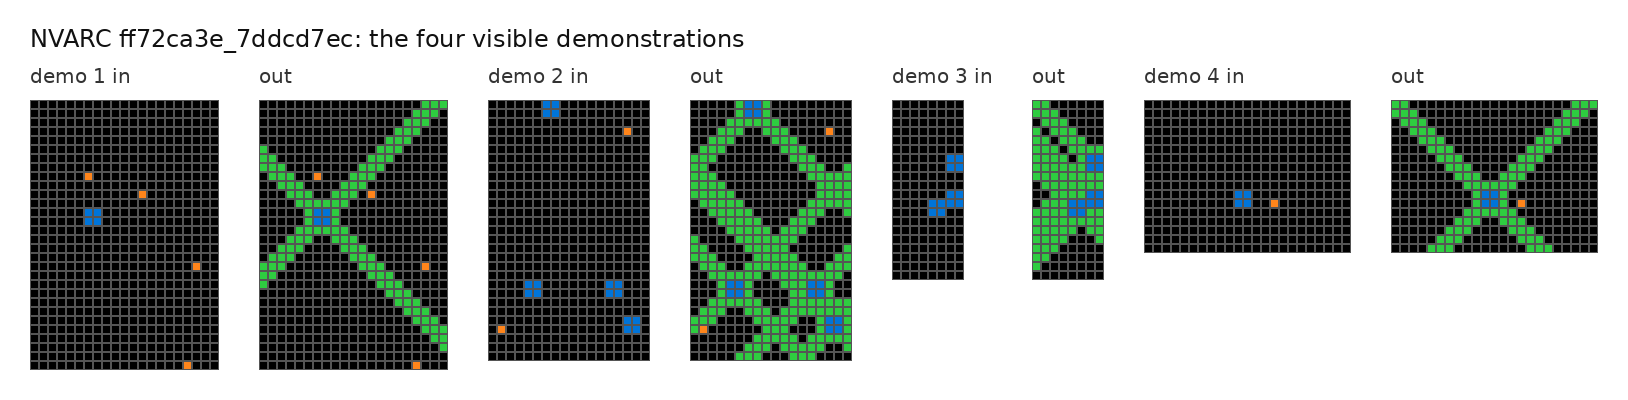
\includegraphics[width=\linewidth]{fig-nvarc-ff72ca3e-demos.png}\\[0.5em]
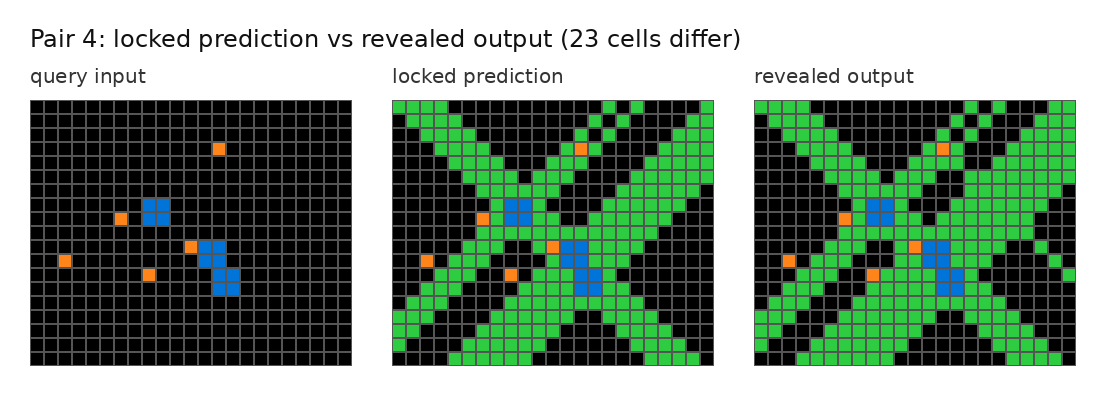
\includegraphics[width=\linewidth]{fig-nvarc-ff72ca3e-reveal.png}
\caption{NVARC \texttt{ff72ca3e\_7ddcd7ec}. Top: the four visible
demonstrations. Bottom: the query input, the locked prediction, and the revealed
output, which continues rays at orange cells.}
\label{fig:nvarc}
\end{figure}

\paragraph{How often a drawn lesson hides it.} Let $c=13$ of the puzzle's
$n=30$ pairs be consistent with the simpler rule and $b=17$ not. If a training
sample draws $d$ demonstrations and one query uniformly without replacement, the
probability that every demonstration is consistent with the simpler rule while
the query is not is
\[
  P_d \;=\; \frac{\binom{c}{d}}{\binom{n}{d}}\cdot\frac{b}{n-d},
  \qquad P_3 = 4.4\%,\quad P_4 = 1.7\%,\quad P_5 = 0.6\%.
\]
Such a lesson is supervised to an answer its demonstrations do not determine.
A generator with a lesson schedule (Section~\ref{sec:sampling}) instead places
the distinguishing input in every window by construction, and
\texttt{lesson\_identifiable} rejects the lesson if a declared rival survives,
when export chooses the demonstration count.

\paragraph{Scope.} The audit covered 16 NVARC puzzles. Recorded verdicts: 9
consistent, 1 ambiguous (this case), 1 trivial (output independent of the
rule's structure, pending external adjudication), and 5 without a parsable
verdict. Sixteen puzzles do not support a population error rate, and we do not
claim one.

\paragraph{Ambiguity in our own lessons, kept as a task.} Reviews of ARCpuzzles
generators found the same failure in our own lessons: a retained lesson whose
demonstrations fit a second rule that changes the query answer. The generator
was then repaired so that its schedule shows the distinguishing input, and the
original lesson was kept. Such lessons form a separate auxiliary set,
\emph{find another valid answer}: the prompt shows the demonstrations, the query
and one valid rule with its answer, and asks for a different rule that also fits
every demonstration, and for that rule's answer. Both rules are Racket programs.
A candidate is published only after both run, through the same protected bridge
as the reference rules, on every demonstration and on the query, and are
certified to fit every demonstration and to disagree on the query. The current
snapshot holds 18 certified candidates from 10 generators: 17 lesson groups, 35
prompts, 160 Racket evaluations, none quarantined. The rule pairs are ones a
solver can plausibly confuse: four- versus eight-connected components, enclosed
versus small zero regions, at least one versus exactly one overlap, Manhattan
versus Chebyshev or Euclidean distance, a column count versus the same count
capped at two (Figure~\ref{fig:alt}). The set was copied to the training host
but never trained.

\paragraph{Ambiguity flagged while describing errors.} The agents that
wrote the refine sentences (Appendix~\ref{app:supervision}) checked every
candidate second rule against every demonstration before calling an answer
ambiguous. Among the model's described answers they flagged:

\begin{center}
\small
\begin{tabular}{lrr}
\toprule
Library & Answers described & Flagged ambiguous \\
\midrule
ARCpuzzles & 10,132 & 45 (0.44\%) \\
ARC-GEN & 4,756 & 13 (0.27\%) \\
RE-ARC & 2,649 & 5 (0.19\%) \\
\bottomrule
\end{tabular}
\end{center}

\noindent A recheck of 20 flags confirmed 16, overturned 2 and found 2 coverage
gaps; 43 were not rechecked. Separately, agents described 600 correct outputs
with no model answer involved, drawn from all four libraries, and flagged 12:
6 of 180 NVARC, 4 of 300 ARCpuzzles, 1 of 60 ARC-GEN and 1 of 60 RE-ARC. The
described answers are the model's own attempts, chosen by the training loop, so
these are not population rates, and the counts are too small to rank the
libraries.

\begin{figure}[H]
\centering
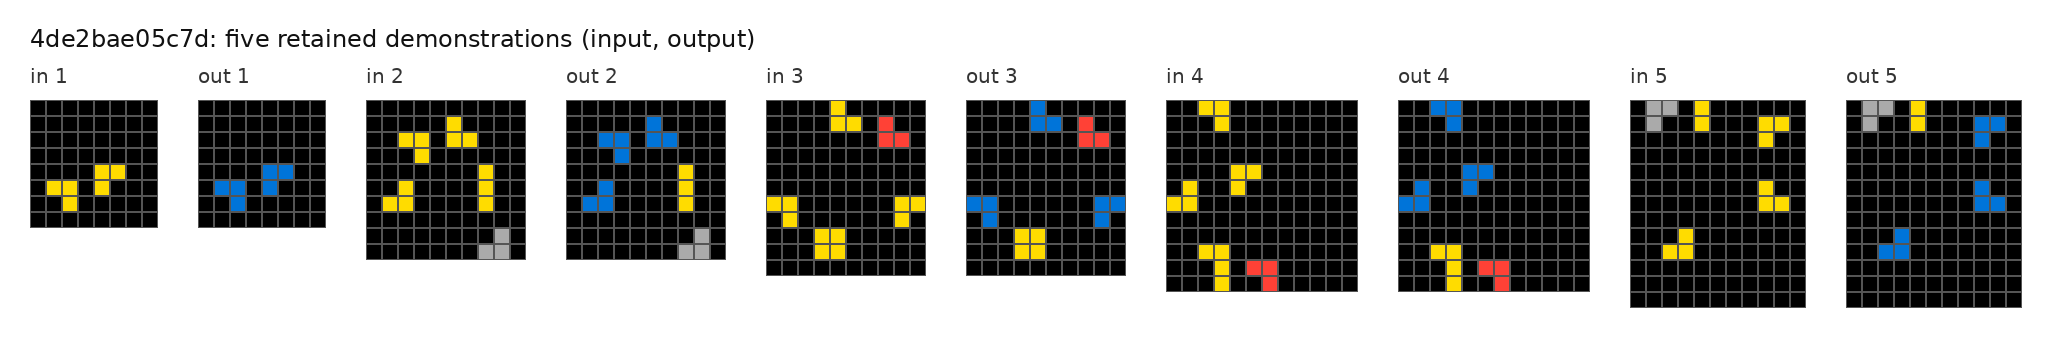
\includegraphics[width=\linewidth]{fig-alt-4de2bae05c7d-demos.png}\\[0.5em]
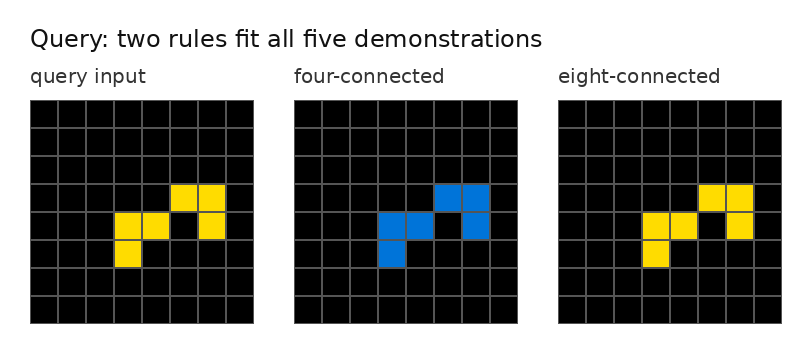
\includegraphics[width=0.62\linewidth]{fig-alt-4de2bae05c7d-query.png}
\caption{A retained pre-repair lesson of \gen{4de2bae05c7d} (recolour yellow
L-triomino components blue). Every demonstration fits both four- and
eight-connected components. In the query two L-triominoes touch only at a
corner: four-connected, they are two L shapes and turn blue; eight-connected,
they are one six-cell component and stay yellow. The repaired generator makes
every five-draw window include such a diagonal contact.}
\label{fig:alt}
\end{figure}

\section{Ideas and pitfalls}
\label{sec:pitfalls}

We list the ideas we used and the pitfalls we hit, each with the case in this
paper that shows it, to help others establish practice for generating this kind
of data. It is what we learned, not a claim that the list is complete or that
our choices are the best ones.

\paragraph{Kinds of work.} Building the data took several distinct kinds of
work, done by the author and by AI agents:
\begin{center}
\footnotesize
\begin{tabularx}{\linewidth}{>{\raggedright\arraybackslash}p{2.6cm}X>{\raggedright\arraybackslash}p{4.2cm}}
\toprule
Work & What it involves & Recorded amount \\
\midrule
Writing rules & Racket reference rules to one written standard; parametric settings & 4,061 generators; 941 families with 2,174 settings \\
Writing samplers & Python input samplers: axes, textures, invariants, schedules & one per generator \\
Attacking rules & Rival rules, witnesses, shortcut searches on the original pairs & 6,822 rivals in 1,498 generators; 4,890 shortcut hypotheses checked in July \\
Reviewing and repairing & Review packets, repairs, new prototypes & 693 reviews in July; 569 records in October (201 repairs, 291 new prototypes) \\
Solving blind & Solving a task before reading its rule, and again after repair & 2,638 attempts on 1,425 generators \\
Auditing & Adversarial findings bound to the source they were found against & 2,472 open findings on 1,748 generators \\
Building checks & The twelve-stage battery, the semantic gate, the lesson census & 12 stages, each from a defect found by hand \\
Engineering & Shared runtime, export, provenance and hashing & about 3,500 commits, 26 March to 2 November \\
Describing errors & One checked sentence per model error, for training & 17,537 answers \\
\bottomrule
\end{tabularx}
\end{center}

\paragraph{Ideas.}
\begin{enumerate}[nosep,leftmargin=1.6em]
  \item Compute every label by executing a reference rule; never author an output (Section~\ref{sec:generator}).
  \item Key each random choice by name, so that adding or changing one draw does not shift the others (Section~\ref{sec:sampling}).
  \item Turn the sample index into a lesson schedule, so that every window of consecutive draws holds the inputs that refute the rivals (Section~\ref{sec:sampling}).
  \item Write rival rules as executable functions, tie each to the input feature that refutes it, and reject a lesson that a rival survives (Section~\ref{sec:rivals}).
  \item Search the original task's own pairs for shortcuts that fit them all, and require generated inputs on which each fails (Section~\ref{sec:rivals}, Appendix~\ref{app:rivals}).
  \item Declare the textures that teach a rule and the textures that hide it (Section~\ref{sec:textures}).
  \item Make a rule parametric: one sampler, several executable settings, and a certificate that each episode's demonstrations leave exactly one setting (Section~\ref{sec:parametric}).
  \item Replay original inputs at a known rate to anchor the distribution, and measure what that costs in effective size (Section~\ref{sec:reach}).
  \item Expose only exact, observable axes, and measure reach (distinct draws, Chao1, $N_{\mathrm{eff}}$) instead of multiplying declared axes (Section~\ref{sec:reach}).
  \item Grow the check battery from defects found by hand (Section~\ref{sec:battery}).
  \item Bind approval to source hashes, and keep every finding attached to the source it was found against (Sections~\ref{sec:release} and~\ref{sec:review}).
  \item Start each review with a blind solve, committed before the reviewer reads the rule (Sections~\ref{sec:review} and~\ref{sec:blind}).
  \item Keep ambiguous lessons as a separate ``find another valid answer'' task instead of discarding them (Section~\ref{sec:blind}).
  \item Keep answers in private files, apart from the model-visible challenges (Section~\ref{sec:use}).
\end{enumerate}

\paragraph{Pitfalls.}
{\footnotesize
\begin{xltabular}{\linewidth}{>{\raggedright\arraybackslash}p{3.5cm}X>{\raggedright\arraybackslash}p{3.3cm}}
\toprule
Pitfall & Case in this paper & What helped \\
\midrule
\endhead
Advertised axes that do not vary anything observable & The imported \gen{5573cf8e2aa4} declared nine axes, several singleton, aliased or inert. Declared configurations and measured reach disagree both ways: 3 declared and 99,997 distinct in 100,000 draws; 196 declared and exactly 2,376. & Expose only observable axes; measure reach \\
\addlinespace
Imitating the originals teaches their shortcuts & Five of the six sampled generators have a rival that fits every original pair, test included, so it scores perfectly on the original task; every original of \gen{fae242ae157d} uses areas 4/5/6 in scan order. & Rivals with generated counterexamples; mass where rule and shortcut disagree \\
\addlinespace
Independent sampling can omit the distinguishing input & An NVARC puzzle hides its second rule from 4.4\% of three-demonstration lessons; \gen{5ca74a85bc85}, with no schedule, produced 4 ambiguous lessons in 60. & Lesson schedules; a per-lesson identifiability check \\
\addlinespace
Fewer demonstrations, more ambiguity & The external screen flags 6.7\% of our two-demonstration episodes and 1.2\% of the rest. & A higher minimum count; certify every lesson \\
\addlinespace
A certificate covers only the rivals it lists & The parametric certificate separates a family's own settings, not generic rivals such as a constant output size. In round 38, 17 of 801 two-demonstration parametric episodes (2.1\%) show outputs of one size while a query needs another, against 5 of 4,355 (0.1\%) with more demonstrations and 26 of 4,014 (0.6\%) from ordinary generators. In one episode of \gen{4dd0b3ed33ee} both outputs are $8\times9$ and three of four queries need $9\times10$ or $7\times8$. & Add generic rivals (constant size, constant colours) to every check \\
\addlinespace
A fixed demonstration count bypasses rejection & With an explicit count the worker keeps a failing lesson and only flags it; the census, which fixes the count, kept 4 ambiguous lessons of \gen{5ca74a85bc85}. & Read the lesson check in the provenance; drop flagged lessons \\
\addlinespace
Subsampling sample indices breaks schedules & \gen{5573cf8e2aa4} places a canonical anchor at every third index; its notes warn that a loader selecting one residue class of indices could bias the curriculum. & Keep indices consecutive \\
\addlinespace
Replaying originals concentrates the distribution & \gen{5ca74a85bc85} replays originals in 18.5\% of draws: $N_{\mathrm{eff}}=146$ while Chao1 exceeds 62,000. & Measure $N_{\mathrm{eff}}$; choose the replay weight deliberately \\
\addlinespace
A declaration can be wrong & 356 approved generators copy their whole rival list into \texttt{CANONICAL\_SHORTCUTS}; \gen{5573cf8e2aa4} and two of five others sampled fail the fit check. & Verify every declaration by execution \\
\addlinespace
Approval does not follow a stricter check & The fit check arrived on 23 October; generators approved on 3 October and unchanged since fail it. None of the six sampled approved generators passes all twelve stages of today's battery (Section~\ref{sec:battery}). & Re-run new checks on approved generators; record the check version with each approval \\
\addlinespace
An override can leave the rule's domain & \gen{c4f6a0585dbf}: \texttt{palette\_kind=warm} yields inputs its rule leaves unchanged. & Test every override path; keep audits open until resolved \\
\addlinespace
A hidden table can ask for what no demonstration shows & \gen{03478139591b} maps colours by a fixed table (3$\to$1, 5$\to$4, 8$\to$2); a query whose colour no demonstration maps needs an output colour nobody has shown. Over round 38, 21 of 9,170 episodes (0.23\%) have a query needing a colour absent from every demonstration output and from its own input. & Require each table entry a query uses to appear in a demonstration \\
\addlinespace
Originals can break the target format & 13 bank originals have a grid larger than 30. & Validate size limits at import \\
\addlinespace
Label agreement is not identifiability & An NVARC puzzle passes 15-of-20 program agreement and admits two rules on its first four demonstrations. & Check labels and lessons separately \\
\addlinespace
Grid text can merge under the tokenizer & With letter labels, \texttt{(R, C)} merges in 19,800 of 21,600 contexts. & Check token boundaries on every training example \\
\addlinespace
Progress on trained generators overstates generalization & Mastery is measured on fresh draws of generators the model trained on; public-evaluation tasks were in training. & Keep held-out sets; record exposure \\
\bottomrule
\end{xltabular}}

\section{What is released}
\label{sec:release}

The data is large. The library holds 4,061 generators, against 400 in RE-ARC
and about 900 in ARC-GEN; the 1,984 approved ones alone are about five times
RE-ARC and twice ARC-GEN. 941 parametric families add 1,233 Racket rule
variants on top. Each generator is a function of a seed and draws new
instances without a fixed limit; Section~\ref{sec:reach} measures how many
distinct instances six random ones reach.

We release all of it rather than a curated top subset: every generator,
finished or not, with its label, notes, review evidence, counterexamples and
tests. Users choose by label. The unfinished generators show every stage a
generator passes through, from imported and unverified, to machine-checked, to
reviewed and repaired, to approved, so the release documents the curation
process and not only its output. They also show how much work remains to
represent these tasks well: 2,077 generators are not approved, and 1,748 carry
an open finding. Everywhere else, the paper describes only the 1,984 approved generators.
\todo{release link.}

\begin{table}[H]
\centering
\small
\begin{tabularx}{\linewidth}{Xr}
\toprule
Item & Count \\
\midrule
Generators (per-puzzle 4,012; generic 49) & 4,061 \\
\quad approved for training & 1,984 \\
Canonical puzzle rows (original pairs, all variants) & 4,472 \\
Sources: puzzle bank, ARC-AGI-2 training and public evaluation, custom (Table~\ref{tab:sources}) & 4,061 \\
Accepted parametric families (settings) & 941 (2,174) \\
Reviewer solve attempts; standing-question answers & 2,638; 632 \\
Certified ``find another valid answer'' candidates & 18 \\
\bottomrule
\end{tabularx}
\caption{Contents of the release.}
\label{tab:release}
\end{table}

\paragraph{Labels.} Every generator carries a review label and a derived
approval:
\begin{center}
\small
\begin{tabularx}{\linewidth}{lrX}
\toprule
Label & Generators & Meaning \\
\midrule
\texttt{reviewed\_safe} & 1,994 & a reviewer rated training suitability 3 or 4 of 4, or a reviewer's repair was accepted \\
\texttt{reviewed\_standard} & 57 & a reviewer rated suitability 2 of 4 \\
\texttt{provisionally\_safe} & 584 & a repair was returned, or machine checks passed (clean self-check, pinned rule hash, at least 95\% valid draws) without review \\
\texttt{unverified} & 1,007 & no review, and the independent monitor gate is stale or missing \\
\texttt{unsafe} & 415 & an active semantic veto, a failed independent gate, or a machine suitability of 1 or less; mostly machine flags, not review findings \\
\texttt{unreviewed} & 4 & no record \\
\bottomrule
\end{tabularx}
\end{center}
A generator is \emph{approved} when it is \texttt{reviewed\_safe}, its generator
file matches the reviewed SHA-256 exactly and its rule matches the reviewed
hash after whitespace normalization, it has a canonical rule and a
positive mix weight, and no semantic veto is active. Reasons for non-approval
overlap: 2,067 are not reviewed safe, 56 changed code and 15 changed rule after
review, 48 have no canonical rule, 15 have zero mix weight, 4 lack a reviewed
hash and 2 carry a veto.

\paragraph{Open audits.} A finding against a generator stays attached to the
source it was found against until someone resolves it; a later edit does not
clear it. 1,748 generators, 734 of them approved, carry at least one finding
that is not closed. Of the 2,472 open findings, 1,674 await triage, 789 are
unresolved and 9 need evidence. A finding does not revoke approval by itself.
\texttt{arcpuzzles list --audit-unresolved} lists these generators and
\texttt{show ID} gives each finding with its reproduction. For example, an
audit of \gen{c4f6a0585dbf} reproduced that one of its overrides
(\texttt{palette\_kind=warm}) yields inputs its Racket rule leaves unchanged.

\paragraph{Originals outside ARC's size limit.} Thirteen bank puzzles, two of
them with approved generators, have an original grid wider or taller than 30, so
they are not valid ARC tasks and \texttt{show --challenge} refuses them. Their
generators can still draw legal grids: \gen{6c68e1b008a5}, whose original is
$9\times59$, draws inputs at most 29 wide.

\section{Exporting training data}

\texttt{arcpuzzles export} samples only approved generators by default, either
in proportion to each generator's mix weight or uniformly; seeds and the full
pool are recorded. An episode can carry four supervised queries over one shared
set of demonstrations, all under the same rule and setting. Query answers are
written to private files, never to the model-visible challenge file. Each row
records the generator hash and its verified original-task family, or marks the
family unknown; no train/evaluation split is invented.

\section{Using the release}
\label{sec:use}

Querying needs only Python 3.12 or later. Generation and checks also need
Racket on the path (or \texttt{RACKET\_PATH}), NumPy and Pillow. A portable
bundle pins approved sources with a Linux Racket for machines without one.

\noindent\begin{minipage}{\linewidth}
\begin{lstlisting}
python3 -m venv .venv && . .venv/bin/activate
pip install -e '.[runtime,dev]'
arcpuzzles stats                                  # counts and labels
arcpuzzles list --approved --source training --limit 20
arcpuzzles show 3ef9eae12446 --challenge          # demonstrations, no answers
arcpuzzles generate 3ef9eae12446 --count 2 --seed 17 --train 2 --test 1 \
    --out var/examples.jsonl
arcpuzzles export --approved --count 4 --seed 17 --sampling uniform \
    --style episodes --out var/datasets/approved-s17
arcpuzzles export --parametric-only --count 4 --seed 17 --sampling uniform \
    --style episodes --out var/datasets/accepted-s17
arcpuzzles inspect-export var/datasets/approved-s17
arcpuzzles check 3ef9eae12446 --battery --out var/checks/3ef9  # 12 stages
arcpuzzles lesson-census 3ef9eae12446 --per-band 20 --out var/census/3ef9.json
\end{lstlisting}
\end{minipage}

\begin{itemize}[nosep]
  \item \textbf{Train on approved generators.} Generation and export refuse unapproved generators by default. \texttt{--allow-unapproved} opens them for research and labels every output as unapproved.
  \item \textbf{Keep answers private.} Exports write the model-visible challenges and the private labels to separate files; the labels must never enter the challenge file.
  \item \textbf{Read the provenance.} Every episode carries its seed, sample indices, executed rule hash, rejections and lesson check. With a fixed demonstration count, drop episodes whose check is \texttt{diagnostic\_unsupported}.
  \item \textbf{Keep sample indices consecutive.} A lesson schedule is a function of the sample index; a loader that keeps one residue class of indices can remove the inputs that refute the rivals.
  \item \textbf{Check open audits} before relying on a generator, and decide whether its finding matters for the use at hand.
  \item \textbf{To continue a generator}, start from its \texttt{notes.md}, counterexamples and tests, run the battery, and treat its label as a claim about the reviewed bytes only.
\end{itemize}

\section{Submission}

Our ARC-AGI-2 submission is a Qwen3.8-27B that writes the output grid directly,
trained for 273 GPU-hours (231 on one GPU, 42 on two rented multi-GPU pods) on
training examples drawn almost entirely (94\%) from generators:
ARCpuzzles plus screened RE-ARC, ARC-GEN and NVARC episodes. The run, its
supervision format and its evaluations are in the appendices
(\ref{app:run}--\ref{app:agent}). \todo{final public leaderboard score and
submission ID.} The 2026 third-place solution trained on far more data: it
reports about six million verified puzzles, each expanded
into 24 augmented samples \cite{darragh2026}. We do not attribute the accuracy
gap to data volume alone; model, format, test-time training and compute differ.

\section{Conclusion}
\label{sec:conclusion}

Labels computed by an executable rule are correct by construction, so the hard
part of building data for ARC is the lesson: which inputs appear together, and
whether they rule out the readings a solver would plausibly take instead. No
finite lesson determines a rule, so every lesson check here is relative to
declared rivals, a regularizer rather than a proof. Within that frame,
the measurements in this paper say where lessons fail. Simple shortcuts fit the
original pairs of five of six randomly sampled generators. In one audited NVARC
puzzle, independent sampling hides a second rule from 4.4\% of
three-demonstration lessons. Two-demonstration
episodes are flagged several times as often as longer ones. Declarations and
approvals drift as the checks tighten: none of six sampled approved generators
passes today's battery in full.

We release all 4,061 generators, unfinished ones included, with their labels,
open findings and evidence, so that others can use the approved ones, see how
much work remains, and continue it. Section~\ref{sec:pitfalls} lists the ideas
and pitfalls we would want to know before starting again.

\section{Limitations}
\begin{itemize}[nosep]
  \item Rival and identifiability checks cover declared rivals on sampled lessons; they do not prove uniqueness.
  \item Approval binds a generator's source hash, not the gate version. Checks added later, such as the 23 October verification of declared canonical shortcuts, are not re-run on approved generators; three approved generators examined here fail it.
  \item ARCpuzzles episodes were not filtered by the external identifiability screen of Table~\ref{tab:screen} during training. Applied afterwards to a random 1,000 of them, it flags an ambiguous query in 1.8\% (Table~\ref{tab:screen-ours}).
  \item Most review results are reviewer-reported and were not re-run when integrated.
  \item The 415 \texttt{unsafe} labels are not a review-measured defect rate. A generator is \texttt{unsafe} when it has an active semantic veto, failed an independent monitor gate, or, before any review, has a machine-estimated suitability tier of 1 or lower. Unsafe generators are excluded from training exports.
  \item 120 generators were written for ARC-AGI-2 public evaluation tasks, and the submission's training run included 3,981 training examples from public evaluation tasks. Local public-evaluation scores of that model are therefore not held-out measurements; the competition's hidden test tasks are separate.
\end{itemize}

\begin{thebibliography}{9}
\bibitem{v01} R.~Kirk. What's all the Racket about? ARC-AGI-2 generators, v0.1. \url{https://github.com/definitelynotrussellkirk-bit/arc-agi-2-generators}, May 2026.
\bibitem{chollet2019} F.~Chollet. On the Measure of Intelligence. arXiv:1911.01547, 2019.
\bibitem{arcagi2} F.~Chollet et al. ARC-AGI-2: A New Challenge for Frontier AI Reasoning Systems. arXiv:2505.11831, 2025.
\bibitem{arcprize2025} ARC Prize 2025: Technical Report. arXiv:2601.10904, 2026.
\bibitem{rearc} M.~Hodel. Addressing the Abstraction and Reasoning Corpus via Procedural Example Generation. arXiv:2404.07353, 2024. \url{https://github.com/michaelhodel/re-arc}.
\bibitem{arcgen} ARC-GEN: a mimetic procedural benchmark generator for the Abstraction and Reasoning Corpus. arXiv:2511.00162, 2025. \url{https://github.com/google/ARC-GEN}.
\bibitem{nvarc} I.~Sorokin and J.-F.~Puget. NVARC solution to ARC-AGI-2 2025. \url{https://github.com/1ytic/NVARC}.
\bibitem{darragh2026} Darragh and CPMP. [ARC-AGI-2] Public 3rd Place Solution. Kaggle, 2026. \url{https://www.kaggle.com/competitions/arc-prize-2026-arc-agi-2/writeups/arc-agi-2-public-3rd-place-solution}.
\end{thebibliography}


\appendix

\section{The submission training run}
\label{app:run}

Direction was set on 22 October 2026: one Qwen3.8-27B answering with the grid
directly, thinking disabled; everything trains, with no hold-out except
generators approved after a round was frozen; and no puzzle trains twice, so
each training example is a fresh generator instance. A \emph{route} is one training example: a prompt
and its supervised answer turns, in one of the modes of
Appendix~\ref{app:supervision}.

\begin{table}[H]
\centering
\small
\begin{tabularx}{\linewidth}{lX}
\toprule
Model & Qwen3.8-27B, LoRA rank 128, thinking off \\
Optimiser & one AdamW kept across rounds: LR $10^{-4}$, betas (0.9, 0.95) to round 13; $1.5\times10^{-4}$, (0.9, 0.98), 28 routes per update from round 14; $7\times10^{-5}$, 112 routes per update and $\beta_2=0.99$ by round 25 (decided 28 October, when training loss had flattened) \\
Schedule & 48 continual rounds, 22 October -- 2 November 2026 \\
Training time & 231.4 GPU-hours on one RTX PRO 6000 across 42 rounds, plus 41.6 on rented 4- and 8-GPU pods (Table~\ref{tab:burst}) \\
Global updates & about 19{,}970 by 2 November \\
Round datasets & 379,598 admitted routes \\
\quad from generators & 358,387 (94.4\%) \\
\quad from public training tasks & 17,230 \\
\quad from public evaluation tasks & 3,981 \\
Routes by mode & direct 207,625; refine 70,092; verify-then-fix 55,461; verify 27,304; points 14,079; fix 3,597; exec 1,440 \\
Parametric families & from round 7; up to 292 families and 623 settings in one round \\
External generators & RE-ARC 391, ARC-GEN 891, NVARC 855 files, requested at one third of generator items \\
Pilot (round 1) & 4,332 episodes from 1,459 approved generators in 530 families; answer loss 0.191 $\to$ 0.124 \\
\bottomrule
\end{tabularx}
\caption{The training run.}
\end{table}

\begin{figure}[H]
\centering
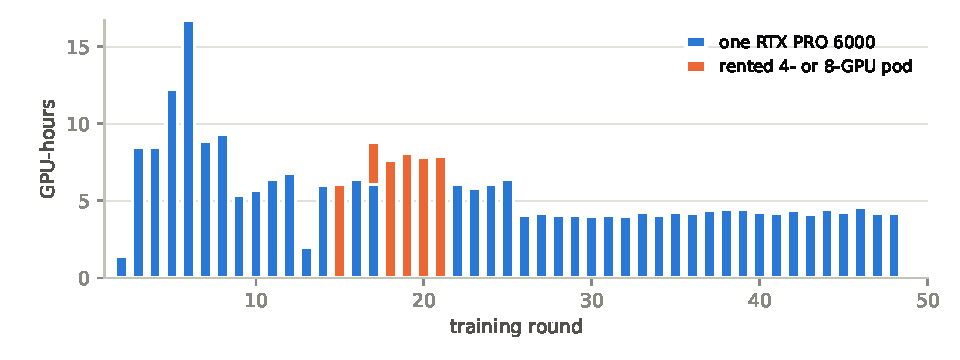
\includegraphics[width=\linewidth]{fig-run-hours.pdf}
\caption{GPU-hours trained per round. Blue: the single RTX PRO 6000. Orange:
rented pods (Table~\ref{tab:burst}), as GPUs times trainer seconds per round,
round switches excluded (40.1 GPU-hours; 41.6 including switches). Round 17
was split between the two. Round 49 was still training.}
\end{figure}

\paragraph{Burst runs on rented GPUs.} The main run trained on one RTX PRO
6000 (Blackwell, 96\,GB) at about 2,000 processed tokens per second. On 26--27
October we tried three rented bursts that continued the same LoRA, optimiser
state and global update count on prepared rounds, then handed a verified save
back to the main run:

\begin{table}[H]
\centering
\small
\begin{tabularx}{\linewidth}{lrrrrX}
\toprule
Pod & Training & Updates & Tokens/s & vs one GPU & Outcome \\
\midrule
1$\times$ B300 (26 Oct) & 0.2\,h & 27 & 4,870 & 2.4$\times$ & stopped by its cost guard below the speed floor; not adopted \\
4$\times$ RTX PRO 6000 (27 Oct) & 1.49\,h & 199 & 6,824 & 3.4$\times$ & finished round 15; round 16 continued from its save \\
8$\times$ RTX PRO 6000 (27 Oct) & 4.45\,h & 977 & 12,155 & 6.0$\times$ & rounds 17 (rest) to 21; round 22 continued from its save \\
\bottomrule
\end{tabularx}
\caption{Burst runs. Tokens are processed tokens; ``vs one GPU'' compares with
the single-GPU run on the same trainer settings.}
\label{tab:burst}
\end{table}

The 8-GPU pod was rented for about five and a half hours at \$19.92 an hour. It
trained 4.45 hours: 186.6M tokens processed, 40.8M supervised, equal to 25.7
hours of the single GPU. Throughput was 75\% of eight times the single GPU;
the main loss was ranks waiting at the gradient all-reduce for the slowest
rank, because shards were balanced by routes, not tokens (28\% of update time
in the first 552 updates). On the 72 updates whose batches matched the single
GPU's exactly, mean loss was 0.04380 against 0.04406. Its five prepared rounds
were sized from an estimated speed and ran out before its 4.75-hour time stop:
we did not know how much data, or how much time, a longer run needed.

We decided against further burst runs, because we could not tell how much the
model's ability was still increasing per round, and because we were not sure
we would be able to submit.

\begin{figure}[H]
\centering
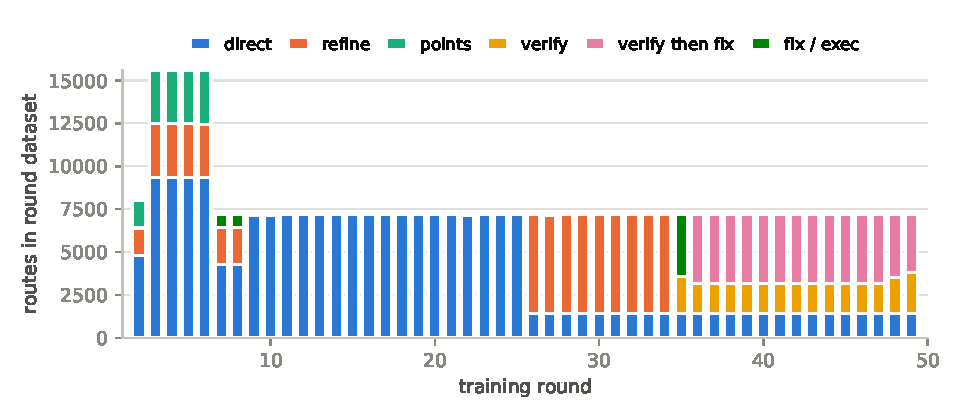
\includegraphics[width=\linewidth]{fig-run-modes.pdf}
\caption{Routes per round dataset by supervision mode. Rounds 2--6 mix direct
answers, refinement of the model's own earlier attempts, and point queries;
rounds 7--8 replace point queries with Racket execution routes;
rounds 9--25 are direct only; rounds 26--34 are mostly refinement; round 35
splits repair into verify and fix; from round 36
the model first verifies a previous answer and, if it is wrong, writes the whole
correct grid.}
\end{figure}

\section{Supervision format}
\label{app:supervision}

Supervision changed several times during the run (format versions 2 to 8). The
final format has these parts.

\paragraph{Labelled grids.} Every grid begins with a name line (\texttt{train 1
input, size 26x21}). The next line is a column ruler: \texttt{i} for an input or
\texttt{o} for an output, a bar, and one label per column. Every row begins with
its row label and a bar. Labels run from 0 to 29 using one character each, so
that each label is one token and rows and columns stay aligned:
\texttt{0123456789aBcDfEgHjIqkLpNtOvUw}. A cell is written \texttt{\textasciitilde
R|C} for row label $R$ and column label $C$; \texttt{\textasciitilde c|4} is
cell $(12,4)$. Labels were added on 23 October so the model can locate cells
instead of counting rows; the one-token constraint followed on 24 October.

\paragraph{Nothing merges under the tokenizer.} Every character of a size line,
a column ruler, a labelled row, a cell reference and a label list is exactly one
token, in every context where it appears. The build checks this on the stored
token ids of every training route and evaluation prompt and fails on any
violation. The Qwen tokenizer keeps the digits 0--9 separate, so each cell of a
row is one token. Letters merge with their neighbours, so the twenty letter
labels were chosen, in mixed case, so that no two adjacent labels merge; this
was checked for all 900 row--column label pairs. The base model itself writes
cells as decimal tuples, $(12, 4)$, which costs seven tokens; with letter labels
every bracket, comma or space form merges a label into its neighbour. Measured
with the pinned tokenizer over all 900 label pairs, 8 preceding contexts and 3
joins:

\begin{center}
\small
\begin{tabular}{ll}
\toprule
Cell notation & Labels that stay one token \\
\midrule
\texttt{(R, C)} & digits only; 19,800 of 21,600 contexts merge \\
\texttt{(R,C)} & digits only; \texttt{,a} merges \\
\texttt{(R|C)}, \texttt{[R|C]}, \texttt{(R;C)} & digits only; the opening bracket merges with letters \\
\texttt{\textasciitilde R|C} & all 30, unless a space precedes \texttt{\textasciitilde} (the renderers never write one) \\
\bottomrule
\end{tabular}
\end{center}

\noindent \texttt{\textasciitilde R|C} was chosen for exactly this reason: it is the
one form in which no label ever combines with its neighbour. \texttt{\textasciitilde}
plays the opening bracket and \texttt{|} the comma, keeping the model's own
row-first frame with tokenizer-safe glyphs. Of all printable
ASCII, Greek letters and mathematical symbols, only the digits stay separate
after a bracket, a space and a comma; the only alphabets that would survive the
literal tuple are CJK ideographs and fullwidth forms, which carry number
meanings that clash with the colour digits. The ruler corner is a lowercase
\texttt{i} or \texttt{o}, because uppercase \texttt{I} and \texttt{O} are labels
19 and 26 and both stay one token before \texttt{|} (\texttt{>} would merge into
\texttt{>|}). Audits on 24 October found no violation in 1,371,787 and
2,937,294 labelled spans of two rounds, and none in 1,443,329 spans of the first
dataset in the final grid format.

\paragraph{Size and colours first.} An answer states its size, then the colours
it uses, then the ruler and rows. Committing to the output size before any cell
is written was the first format decision (22 October): reading left to right,
every later token is conditioned on a declared shape.

\paragraph{Facts line.} After each test input, a line computed from the shown
grids gives the input's size, colour counts and same-colour shape counts, then
what the train pairs share: whether the size is preserved, the output colours,
colours added or removed, changed cells per pair, the background, and symmetry.
It is about 90 tokens and is the same for every task, so the model has a fixed
place to read structural facts.

\paragraph{Answer facts: extra supervision.} The facts were added for extra
supervision. From 23 October, half of the direct and point routes also ask, at
the end of the user turn, for 2 to 4 facts about the answer, and the target
adds a \texttt{facts} block after the grid or cells: the count of one colour,
that colour's count in each row or column, a colour's bounding box as two cell
references, and similar. Each fact is a name line, then its value, in the same
names and formats as the Facts line and the labelled grid. Values that hold
labels start their own lines, because a preceding space or comma would merge a
letter label into another token. The request never hints at the answer: colour
facts name only colours the prompt shows, and the size and colours that every
answer already states are never asked. The request is part of the prompt so
that the model is conditioned to expect a facts block only when asked. We never
planned to ask for facts at inference; with the request in the prompt, the extra
targets do not teach answers to continue past the grid, and a prompt without a
request keeps the same format at training and at inference. Facts tokens were
3.5--6.4\% of supervised tokens in rounds 6--10, were switched off in rounds
11--25, and were 11--17\% from round 26 (3\% in round 35).

\paragraph{Four queries per prompt.} Only answer tokens carry loss, so a prompt
whose demonstrations are long and whose answer is short supervises little of what
it processes. Rounds 2--4 answered one test input per prompt. From round 5
(23 October) the round builder asks every direct route for four test queries on
one set of demonstrations, given as successive user turns: the demonstrations are
read once and supervise four answers. A route carries fewer only when the
episode's remaining test pairs were already trained, are held for point queries,
or would exceed the token budget. Rounds 4 and 5 have the same mode mix (9,360
direct, 3,120 refine and 3,120 point routes) and the same 15,600 segments, so
they isolate the change:

\begin{center}
\begin{tabular}{lrr}
\toprule
& round 4 & round 5 \\
\midrule
Queries per direct route & 1 & 4 (88\% of routes) \\
Direct answers supervised & 9,360 & 35,828 \\
Tokens processed & 28.6M & 42.7M \\
Tokens supervised & 2.44M & 6.54M \\
Supervised share & 8.5\% & 15.3\% \\
\bottomrule
\end{tabular}
\end{center}

\noindent Processed tokens grew by 1.5$\times$ and supervised tokens by
2.7$\times$. In the direct-only rounds 11--25 the supervised share was
21--24\%. It falls to about 12\% from round 26, when most routes are refine or
verify routes, which show a previous answer and supervise one reply.

\paragraph{Modes.}
\begin{description}[nosep,leftmargin=1.5em]
  \item[Direct.] Demonstrations and a test input; the target is the full answer.
  \item[Refine.] A previous answer is shown; the target is the correct grid, or the same grid when it was already right. Previous answers are always the model's own real attempts on generator puzzles, never synthetically perturbed gold. From round 26 the repair first locates the errors. In round 26 it listed the wrong cells, then their colours. From round 27 an \texttt{error} block opens with the output size, then says \texttt{no error}, or \texttt{wrong size}, or lists every wrong cell as \texttt{\textasciitilde R|C} in row order and only then their count; the whole correct grid follows. Listing the cells before the count, and repeating the full grid after them, gives the model a second chance to emit the grid in order. Before the fix, the target can carry one English sentence on the cause of the error. Claude agents (Opus from 24 October) that see the puzzle's rule, the answer and its wrong-cell map pick one of ten causes (wrong target, missed cells, wrong shape, wrong colour, overreach, wrong size, no change, wrong rule, correct, ambiguous) and write the sentence to a strict guide: colours as \texttt{color N}, cells by their row and column labels, counts in digits. A checker rejects any sentence off the guide. 17,537 of the model's answers were described this way. When another rule also fits every demonstration, the cause is \emph{ambiguous} and the sentence names it (\emph{\dots but another possible rule is \dots}), so the model learns to name a second reading it can use for its second attempt.
  \item[Points.] The prompt lists 9 to 16 cells, or a $3\times3$ to $4\times4$ block, and asks for their values. Since 24 October the answer first states the output size, then the values. Cells are chosen from the hardest available: cells the model got wrong in its attempts, else the highest-loss cells from a prefill scan (Appendix~\ref{app:mastery}), else cells that differ from the input.
  \item[Verify, fix, verify-then-fix.] Round 35 split repair into its two tasks: \emph{verify} shows a previous answer and asks only for the \texttt{error} block; \emph{fix} shows a previous answer with its \texttt{error} block and asks for the whole correct grid. From round 36 both share one prompt: the first turn verifies, and when the previous answer is wrong a follow-up turn asks for the whole correct grid, so one reading of the puzzle trains both tasks. A right previous answer stays a single-turn verify.
  \item[Exec (rounds 7--8).] The demonstrations are replaced by one short instruction and the generator's executed Racket rule, byte for byte; the generator's own inputs follow one per turn, and each answer is the output grid in the ordinary answer block. No examples and no Facts line. 720 routes per round, each from a different generator. The rule is given losslessly as a program, and the short prompt raises the ratio of supervised to processed tokens. Dropped from round 9, when the mix became all direct.
\end{description}

A point query from round 6, with the prompt's grids omitted:
\begin{lstlisting}
Facts: test 24x25; counts 5:598 8:1 9:1; objects 5:1 8:1 9:1. demos 4;
size rule same; out 0 1 3 4 5 6 7 8 9; added none; removed none;
changed 24 14 20 18; bg 4; symmetry none.

Cells:
~k|7~k|8~k|9~L|7~L|8~L|9~p|7~p|8~p|9
--- target ---
```cells
24x25
9 5 5 5 5 5 5 5 5
```
\end{lstlisting}

The start of a direct answer from round 48:
\begin{lstlisting}
Facts: test 1 input size 26x16; counts 0:176 1:2 2:2 6:2 7:180 8:2 9:52;
shapes 1:2 2:2 6:2 7:15 8:2 9:15. train pairs 4; size rule same; output
colors 0 1 2 3 4 5 6 7 8 9; added none; removed none; changed cells per
train pair 10 4 4 6; bg 0; symmetry none.
--- target ---
```grid
size 26x16
colors: 0 1 2 6 7 8 9
o|0123456789aBcDfE
0|0000000000000000
1|0777707777077770
2|0729707297072970
...
```
\end{lstlisting}

\section{Late-round evaluations}
\label{app:evals}

Adapters from the last training days were evaluated on Slurm with one sample per
item. Public evaluation tasks were in training from round 2, so that panel is
not held out. Fresh panels draw new instances from generators.

\begin{figure}[H]
\centering
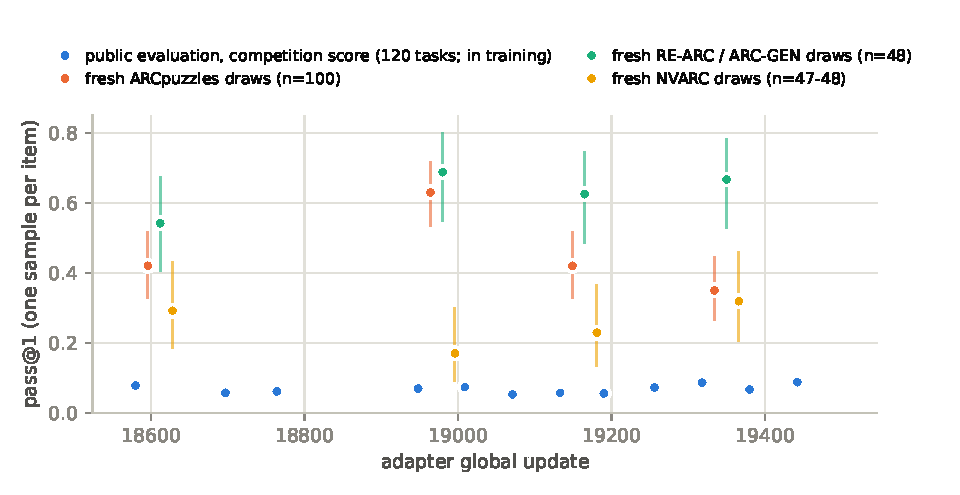
\includegraphics[width=\linewidth]{fig-run-evals.pdf}
\caption{pass@1 by adapter. Public evaluation is the competition-style score
over 120 tasks (any of up to two attempts; here one sample).}
\end{figure}

\begin{table}[H]
\centering
\small
\setlength{\tabcolsep}{4pt}
\begin{tabular}{rrrrrr}
\toprule
Update & Public eval (\%) & Fresh ARCpuzzles & Fresh RE-ARC/ARC-GEN & Fresh NVARC & Retention \\
\midrule
18,604 & 7.78 & 42/100 & 26/48 & 14/48 & 14/48 \\
18,721 & 5.69 & & & & \\
18,788 & 6.11 & & & & \\
18,972 & 6.94 & 63/100 & 33/48 & 8/47 & 11/48 \\
19,033 & 7.36 & & & & \\
19,095 & 5.28 & & & & \\
19,157 & 5.69 & 42/100 & 30/48 & 11/48 & 14/48 \\
19,214 & 5.56 & & & & \\
19,280 & 7.22 & & & & \\
19,342 & 8.61 & 35/100 & 32/48 & 15/47 & 20/48 \\
19,404 & 6.67 & & & & \\
19,466 & 8.75 & & & & \\
\bottomrule
\end{tabular}
\caption{The numbers behind the chart. Fresh panels were run on four of the
twelve adapters.}
\end{table}

\section{Prefill scans and per-generator mastery}
\label{app:mastery}

\paragraph{Scanning by prefill.} To find what the model had not learned without
sampling its answers, the gold answer was scored in one forward pass. For a
prompt $p$ and gold answer tokens $a_1,\dots,a_T$ the scan reads
\[
  q_t \;=\; P_\theta(a_t \mid p,\, a_{<t}), \qquad t=1,\dots,T,
\]
from the prompt log-probabilities of the concatenation $p\,a$, and generates
nothing. An item is \emph{mastered} when $\min_t q_t \ge 1/2$. Then no other
token is more likely than $a_t$ at any step, so greedy decoding reproduces the
gold answer (barring an exact tie at $1/2$). Until 23 October the rule was
$\prod_t q_t \ge 1/2$, which marks a long answer hard even when every cell is
confident. Each grid cell is one token, so the $q_t$ of the answer rows form a
loss grid over the cells; a cell with $q_t<1/2$ fails the threshold, although
its gold colour may still be the greedy choice given a correct prefix.

The scans ran in two lanes. The training cluster served the BF16 model with
vLLM and asked for prompt log-probabilities with a one-token completion. Local
RTX 3090 and 4090 cards ran an IQ4 GGUF quantisation through a small C++ program
on libllama (\texttt{prefill\_nll}), at about 870 prefill tokens per second on
the 3090. A scan costs one forward pass per item and no decoding, so the local
cards scored many more items than they could answer. Scans targeted the next
round's export before it trained, so scanned draws were untrained.

\paragraph{How the scans steered the data.}
\begin{itemize}[nosep]
  \item \textbf{Draw order.} The round builder scored each generator draw by gold-answer loss per processed token: the draw's own scan, else its generator's newest scanned mean, else the median. Mastered draws went to the back of the queue, except a seeded 10\% retained; every generator's first kept draw came before any second. A revised generator (new source hash, or new executed rule hash for a parametric setting) did not inherit its old score. Round 38 scored 189,689 draws, kept 12,633 generator draws, moved 2,446 mastered draws back and retained 273.
  \item \textbf{Point queries.} Without a wrong attempt of its own, a point query asks for the scan's highest-loss cells (Appendix~\ref{app:supervision}).
  \item \textbf{A per-generator scoreboard.} Every scan and every greedy answer to an untrained draw was merged into one record per generator.
\end{itemize}

\paragraph{The scoreboard.} By adapter update 18,604 (2 November) it merged 138
scans with 252,766 scored items and 141,432 greedy answers. A generator's class
uses its newest three scan items and newest three answers:
\begin{description}[nosep,leftmargin=1.5em]
  \item[mastered:] at least two recent scan items, all mastered, and no recent wrong answer (with no scan items: at least two recent answers, all right);
  \item[easy:] a recent mastered share or exact-answer share of at least one half;
  \item[hard:] no recent mastery, and on average at least 15\% of answer cells with $q_t<1/2$ (or at least two recent answers, none right);
  \item[unsolved:] at least three observations, never mastered and never answered right;
  \item[medium:] everything else measured.
\end{description}

\begin{table}[H]
\centering
\small
\setlength{\tabcolsep}{4pt}
\begin{tabular}{lrrrrrrr}
\toprule
Library & Generators & Mastered & Easy & Medium & Hard & Unsolved & Unmeas. \\
\midrule
ARCpuzzles (approved) & 1,984 & 473 & 843 & 268 & 305 & 85 & 10 \\
\quad written for public-eval tasks & 120 & 2 & 18 & 21 & 45 & 34 & 0 \\
RE-ARC & 391 & 89 & 166 & 52 & 77 & 7 & -- \\
ARC-GEN & 871 & 310 & 326 & 115 & 91 & 29 & -- \\
NVARC (by source task) & 836 & 44 & 152 & 596 & 20 & 24 & -- \\
\bottomrule
\end{tabular}
\caption{Scoreboard classes on 2 November. Classes are measured on fresh draws
of generators the model trained on: ``mastered'' means new instances of a
trained rule, not a held-out rule. NVARC files are one-offs and count under
their source task. The median ARCpuzzles generator has 115 observations.}
\end{table}

A quarter of the approved ARCpuzzles generators (473) were mastered and two
thirds (1,316) mastered or easy; 390 were hard or unsolved. The 120 generators
written for public-evaluation tasks were the hardest group: 79 hard or unsolved,
2 mastered. The six generators sampled in Section~\ref{sec:reach}:

\begin{table}[H]
\centering
\small
\begin{tabular}{llrrr}
\toprule
Generator & Class & Scan items & Mastered (all items) & Greedy answers right \\
\midrule
\gen{3ef9eae12446} & mastered & 29 & 96.6\% & -- \\
\gen{7ce16af847d6} & easy & 95 & 54.7\% & 55/80 \\
\gen{fae242ae157d} & medium & 56 & 21.4\% & 25/40 \\
\gen{5573cf8e2aa4} & mastered & 68 & 86.8\% & 42/43 \\
\gen{5ca74a85bc85} & mastered & 61 & 77.0\% & 26/33 \\
\gen{6b88648ff0e0} & easy & 85 & 35.3\% & 31/43 \\
\bottomrule
\end{tabular}
\caption{Scoreboard records of the six sampled generators. ``Mastered (all
items)'' counts every scan item since the generator was first scanned; the class
uses the newest three. For \gen{6b88648ff0e0}, 24 unmastered items had no cell
below $q=1/2$: the miss was in the size or colours line.}
\end{table}

\paragraph{What the model found hard.} Hard and unsolved generators usually
fail narrowly. In ARCpuzzles, RE-ARC and ARC-GEN alike, the median hard or
unsolved generator has 0.9\% of its recent answer cells below $q=1/2$: the
model gets nearly every cell and still not the whole grid. The NVARC median is
16.3\%, because NVARC files received no greedy answers and reach the hard class
only through the cell threshold. Table~\ref{tab:hard-ours} lists the five
ARCpuzzles generators with the largest recent share, all from the puzzle bank;
each asks the model to count or compare objects and write the result into a
small output grid (Figure~\ref{fig:hard-ours}).

\begin{table}[H]
\centering
\footnotesize
\begin{tabularx}{\linewidth}{lXlrrr}
\toprule
Generator & Rule & Class & Scans & Answers right & Cells $q<1/2$ \\
\midrule
\gen{941f7ac13580} & count each object's cells; output the counts in reading order & unsolved & 18 & -- & 60.0\% \\
\gen{b3750af4dac1} & find the room whose area, doors and colour counts match the first room's; mark it in a strip & unsolved & 54 & -- & 44.4\% \\
\gen{6c2353a2cdee} & rotate three templates by their codes, overlay them, colour each cell by how many cover it & unsolved & 78 & 0/81 & 28.0\% \\
\gen{71982ba2b59e} & $N\times N$ matrix relating every pair of objects: same shape up to rotation, same colour, or neither & hard & 83 & 1/69 & 17.8\% \\
\gen{26f313fdf812} & $N\times N$ matrix comparing the areas of every pair of objects & unsolved & 85 & 0/64 & 12.0\% \\
\bottomrule
\end{tabularx}
\caption{The five ARCpuzzles generators with the largest recent share of answer
cells below $q=1/2$, among hard and unsolved generators with at least 8 scan
items, not counting those written for public-evaluation tasks. ``Answers
right'' counts every greedy answer to an untrained draw; ``--'': none was
requested.}
\label{tab:hard-ours}
\end{table}

\begin{figure}[H]
\centering
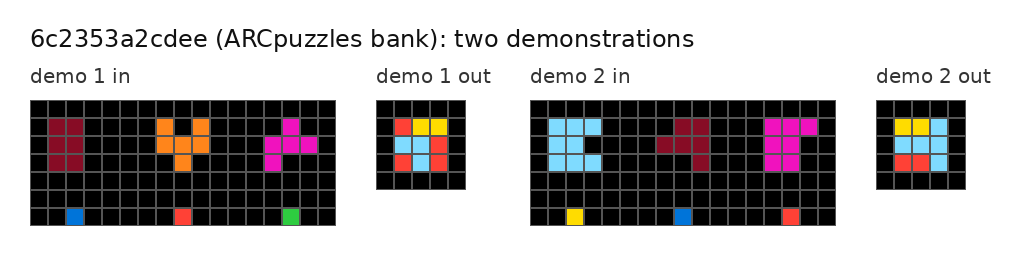
\includegraphics[width=0.8\linewidth]{fig-hard-6c2353a2cdee.png}
\caption{\gen{6c2353a2cdee}, seed 17. The bottom row holds a rotation code
(colours 1--4) under each template; the output overlays the rotated templates
and colours each cell by how many cover it (1 red, 2 yellow, 3 cyan). The model
answered none of 81 draws right.}
\label{fig:hard-ours}
\end{figure}

The same ARC task can be hard in every library's version of it.
Table~\ref{tab:hard-cross} lists ARC training tasks that are hard or unsolved in
at least two of RE-ARC, ARC-GEN and NVARC (26 tasks; eleven shown), with our
generator for the same task. Some are hard everywhere. In \texttt{dc2aa30b},
nine $3\times3$ blocks are sorted by their count of blue cells and laid out from
the bottom row up; the model answered 0 of 58 ARC-GEN draws and 1 of 68 of ours
right (Figure~\ref{fig:hard-dc2a}). Others are hard in RE-ARC and ARC-GEN but
easy in ours (\texttt{36d67576}, \texttt{b782dc8a}, \texttt{e509e548}), or the
reverse: \texttt{8d510a79} is mastered in ARC-GEN and medium in ours. The
versions differ in grid sizes, palettes and how many objects they draw, so a
class gap does not measure lesson quality; it shows that one rule can be easy or
hard depending on how its inputs are drawn.

\begin{table}[H]
\centering
\footnotesize
\setlength{\tabcolsep}{4pt}
\begin{tabular}{llllll}
\toprule
ARC task & RE-ARC & ARC-GEN & NVARC & ARCpuzzles & Our generator \\
\midrule
\texttt{b775ac94} & hard (1/44) & hard (2/35) & medium & hard (0/53) & \gen{dc2c4869445c} \\
\texttt{dc2aa30b} & -- & unsolved (0/58) & unsolved & hard (1/68) & \gen{3108da8bf9e8} \\
\texttt{045e512c} & hard (2/52) & hard (4/57) & -- & unsolved (0/61) & \gen{b2d6e6b60917} \\
\texttt{7df24a62} & unsolved (0/53) & hard (4/58) & easy & hard (1/42) & \gen{c4f6a0585dbf} \\
\texttt{b527c5c6} & hard (5/56) & hard (3/54) & medium & hard (1/16) & \gen{038f266f3acf} \\
\texttt{5c2c9af4} & hard (10/56) & unsolved (0/42) & -- & hard (2/49) & \gen{1d1cffd62646} \\
\texttt{d07ae81c} & unsolved (0/43) & unsolved (0/53) & medium & not approved & \gen{090529973705} \\
\texttt{36d67576} & hard (1/59) & hard (3/56) & medium & easy (9/55) & \gen{089c14df9952} \\
\texttt{b782dc8a} & hard (3/56) & hard (2/55) & medium & easy (9/42) & \gen{44690b1b635f} \\
\texttt{e509e548} & hard (1/55) & hard (4/54) & medium & easy (33/76) & \gen{6c93e8516229} \\
\texttt{8d510a79} & hard (11/59) & mastered (26/56) & unsolved & medium (12/43) & \gen{91ba301501c5} \\
\bottomrule
\end{tabular}
\caption{ARC training tasks hard or unsolved in at least two external
libraries: scoreboard class, with greedy answers right out of answers given.
NVARC files were scanned but not answered. ``--'': the library has no version
of the task. Our generator for \texttt{d07ae81c} is labelled unsafe and was not
trained on.}
\label{tab:hard-cross}
\end{table}

\begin{figure}[H]
\centering
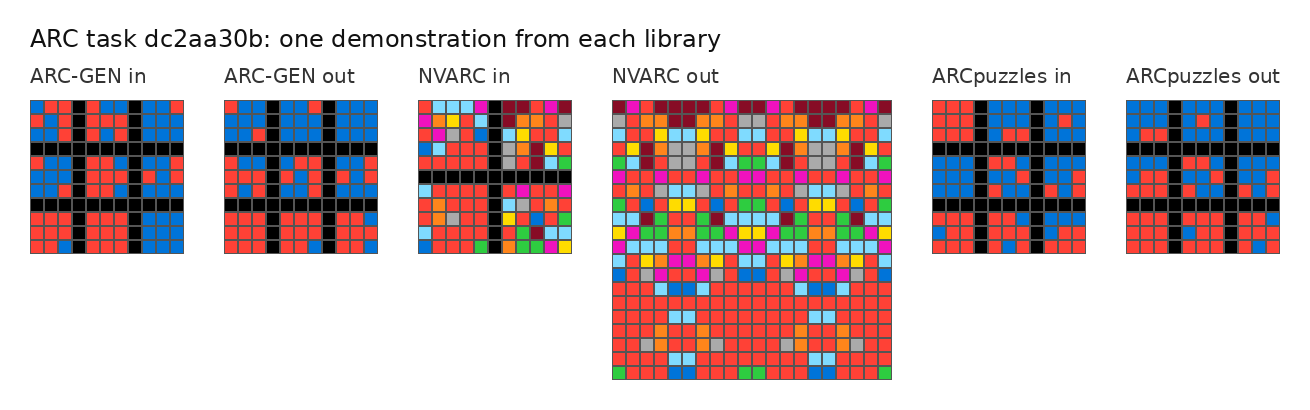
\includegraphics[width=\linewidth]{fig-hard-dc2aa30b.png}
\caption{ARC task \texttt{dc2aa30b}: one demonstration from ARC-GEN, NVARC and
ARCpuzzles (\gen{3108da8bf9e8}, seed 17). The NVARC file is a new puzzle that
NVARC derived from the task, with its own rule ($11\times11$ in, $20\times20$
out); the scoreboard counts it under the task.}
\label{fig:hard-dc2a}
\end{figure}

\begin{figure}[H]
\centering
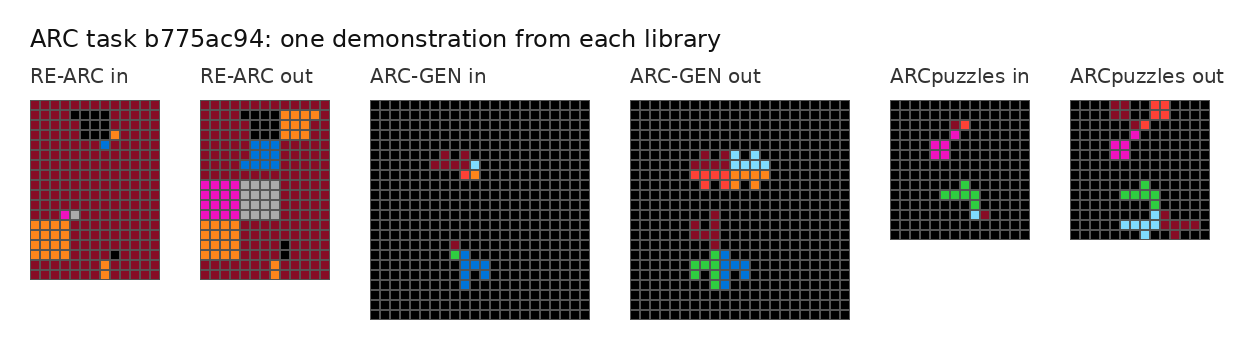
\includegraphics[width=\linewidth]{fig-hard-b775ac94.png}
\caption{ARC task \texttt{b775ac94}: one demonstration from RE-ARC, ARC-GEN and
ARCpuzzles (\gen{dc2c4869445c}, seed 17). A shape is reflected across each side
of its bounding box that a single seed cell marks, in the seed's colour. Hard in
all three.}
\label{fig:hard-b775}
\end{figure}

\section{The 27B agent trace fleet}
\label{app:agent}

Before the direct-grid run, a Qwen3.8-27B tool-using agent (Python sandbox,
thinking enabled) was run on official ARC-AGI-2 tasks across three GPUs
(RTX 3090, RTX 4090, DGX Spark) from 17 to 22 October, recording every token,
log-probability and tool call. These traces were collected for distillation and
were never trained on.

\begin{table}[H]
\centering
\small
\begin{tabular}{lr}
\toprule
Unique episodes & 937 \\
Distinct tasks & 766 \\
Training tasks solved on the hidden test at least once & 542 of 651 \\
Evaluation tasks solved on the hidden test at least once & 46 of 103 \\
Generated tokens & 38.2M \\
Agent turns & 10,245 \\
Stopped by a wall, sandbox, context or episode budget & 126 \\
Slurm jobs; recorded GPU-hours & 30; about 259 \\
\bottomrule
\end{tabular}
\caption{Agent trace collection, deduplicated across mirrors.}
\end{table}

Earlier measurements on the same tasks: the 27B agent solved 33 of the 120
public evaluation tasks, against 3 for Qwen3.5-9B; saved programs from all
models solved 778 of the 1,120 public tasks by 5 October; and an entry combining
NVARC's 4B test-time training with a 27B direct overlay scored 34.86 on the public
leaderboard around 20 October.


\section{Rivals that fit every original pair}
\label{app:rivals}

A canonical shortcut is a rival rule that reproduces every labelled pair of the
original task, training and test, yet differs from the intended rule on other
inputs. At least 761 approved generators declare one or more as literal
dictionaries (209 for ARC-AGI-2 training tasks, 549 for bank puzzles); the
looser text count is 1,223. Each declared shortcut must be checked against every
original pair and paired with generated inputs on which it fails. The fit check
entered the semantic gate on 23 October; Section~\ref{sec:reach} shows approved
generators that copy their whole rival list into the declaration and fail it.

Ten shortcuts drawn at random (seed 20261108) from the 107 documented ones on
approved ARC-AGI-2 training-task generators, quoted from their docstrings:

\begin{table}[H]
\centering
\small
\begin{tabularx}{\linewidth}{llX}
\toprule
Generator & Shortcut & Docstring \\
\midrule
\gen{76aff6297765} & \texttt{profile\_gated\_count\_only} & A curriculum-aware shortcut that exposed the prior four-slot schedule. \\
\gen{9bd5d9c04dd8} & \texttt{most\_non\_eight} & Select the tile with most cells not equal to 8. \\
\gen{4e081a15d785} & \texttt{rowwise\_runs} & Incorrect local run-length encoding; pad ragged results by each row's final colour. \\
\gen{603bd7fff5df} & \texttt{full\_side\_only} & Crop correctly only for continuous sides. \\
\gen{87aae821984d} & \texttt{left\_align\_narrow\_motif} & Bottom-align vertically, but pad narrow motifs right. \\
\gen{a9c4475d7cda} & \texttt{exactly\_two} & Incorrectly treats three as negative. \\
\gen{0ab4fcb302d2} & \texttt{gap\_parity} & Derive the diagonal from gap parity, ignore red. \\
\gen{dbecc530afd0} & \texttt{adjacent\_equal\_row\_pairs\_only} & Pair only adjacent yellow-bearing rows with equal columns. \\
\gen{bf8910eef99b} & \texttt{canonical\_palette\_memorization} & Clip correctly only for palettes memorised from the original data. \\
\gen{92f4d4eb0dbb} & \texttt{inclusive\_midpoint} & Treats an occupied integer midpoint row as the lower half. \\
\bottomrule
\end{tabularx}
\caption{Randomly drawn canonical shortcuts. Rerun against the labelled
original pairs with \texttt{arcpuzzles lesson-census}, each of the ten fits all
of them (3 to 10 pairs per task).}
\end{table}

Some generators record the strongest shortcut in their notes with its
counterexample. Four of them:
\begin{itemize}[nosep]
  \item \gen{dd038eb3d459}: ``use the correct mapping for TR/BR/BL but rotate the green shape 180\textdegree{} for TL. It fits all five available canonical pairs because their only TL green object is a vertical three-cell bar and therefore 180\textdegree-symmetric.''
  \item \gen{be6269bef667}: ``direction 3 continues through color 5 while other directions stop'' fits all five original pairs; the sampler now emits a refuting witness in every draw.
  \item \gen{60a8a9d74a75}: ``fill only enclosed 8-walled regions touched by exactly one colored cell'' fits all five original pairs; on the retained counterexample the intended rule changes 151 cells while the rival changes none.
  \item \gen{aa0b08801e61}: ``memorize the four masks in the public task and map any unknown mask to color 4'' fits all four original pairs; the generator emits novel masks of the same symmetry class.
\end{itemize}

\section{Reviewer instructions (excerpts)}
\label{app:packet}

The October reviewers worked from a packet: a self-contained folder with the
assigned generators, a bundled Racket runtime, tools and written instructions.
The packet is not released. The excerpts below are from the last packet, of
26 October; earlier October packets assigned two or three targets and differed
in detail. Omissions are marked [\dots]; bracketed glosses are ours.

\paragraph{Task statement (\texttt{START-HERE.md}).}
\begin{quote}\small
The current trial is one full parametric build with deep adversarial
self-review. [\dots] Spend the saved second-build effort trying to break your
own artifact: attack shortcut rules and partial intermediates, [\dots] probe
the real minimum lesson and relevant geometry/count/tie boundaries, and
challenge authored certificates [the per-lesson proof that only one setting
fits] and public/private export. Repair findings, retain minimal regressions
and refresh evidence on final bytes. [\dots] Finite checks do not prove
universal uniqueness; keep remaining defects honest. [\dots] No training
admission follows from a reviewer-ready return.
\end{quote}

\paragraph{Lessons and rivals (\texttt{ARC-DESIGN.md}).}
\begin{quote}\small
A single-operation task is legitimate. Do not add operations merely to earn a
category. [\dots] For each applicable axis, identify an actual lesson or
canonical pair [a pair from the original task] and a concrete simpler rival.
Say what observation distinguishes them. A witness [an input on which the
rival and the intended rule disagree] must change the relevant prediction: a
cue that is present but redundant is weak teaching evidence. [\dots]
finite declared-rival checks are not completeness. [\dots] Do not claim corpus
coverage, model mastery or training eligibility from one repair annotation.
\end{quote}
\begin{quote}\small
Make the dependency observable: retain a lawful witness where changing which
object the ray hits changes the later action. Compare with a concrete rival
that skips the hit calculation, such as always selecting the same color or
acting from the emitter alone. Demonstrations should expose the difference.
Merely naming a variable or writing several operations does not establish that
the dependency matters.
\end{quote}

\paragraph{What a parameter may change (\texttt{PARAMETRIC-RULES.md}).}
\begin{quote}\small
Preserve the original reasoning structure: object roles, spatial
relationships, transformations and composition. Prefer a parameter that
exposes a nearby meaningful behavior over a cosmetic reskin or a new unrelated
puzzle. [\dots] Examples include a target or output color, direction, small
count, or threshold. The parameter must change the executed transformation.
Changing only input sizes, object positions, distractors, or sampling weights
does not satisfy this request unless the actual rule also changes. [\dots]
Choose parameter values once per episode from its deterministic seed, then use
the same values for every demonstration and query in that episode. [\dots]
Never resample the hidden rule independently for each pair. Demonstrations
must distinguish the chosen behavior from plausible alternative parameter
settings before a query requires that distinction.
\end{quote}
\begin{quote}\small
[\dots] finite demonstrations cannot prove uniqueness against every imaginable
program. Keep difficult composition and generalization instead of padding every
lesson to defeat arbitrary, contrived rules. [\dots] Inconsistent labels, low
diversity, uncertainty about a rule, and two supported interpretations are
different findings. A reviewer failing to solve a task is not evidence of
ambiguity.
\end{quote}

\paragraph{Ideas for rule diversity (\texttt{PARAMETRIC-EXAMPLES.md}).}
\begin{quote}\small
\textbf{Accepted:} \texttt{f47990415137} selects the component with most
occupied cells, binds its bounding-box aspect ratio, then classifies other
components relative to that ratio. [\dots] Teach occupied-area versus
bbox-area selection with a sparse wide shape and a dense smaller box. Teach
thresholds with below/equal/above-anchor sizes and changing anchors, defeating
fixed-threshold shortcuts.
\end{quote}
\begin{quote}\small
``Ignore'' can mean ineligible for selection, transparent to traversal, or
protected from writes; these are different rules.
\end{quote}
\begin{quote}\small
Use 2--6 demos to distinguish plausible choices, then four private queries
exposed one at a time: transfer, changed geometry/interaction, a relevant
boundary, and substantive 30$\times$30 content where lawful [allowed by the
generator's input rules]. Prefer matched inputs across settings; incidental
layout or palette should not reveal the rule. [\dots] Fit rivals to demos
before inspecting query disagreement. A finite rival bank or native acceptance
[the owner's acceptance of the family] never proves unrestricted uniqueness or
learning benefit.
\end{quote}

\end{document}
